\documentclass[a4paper, oneside, 12pt]{report}
\usepackage[slovene]{babel}
\usepackage[utf8]{inputenc}
\usepackage[left=3cm, top=3cm, right=2.5cm, bottom=2.5cm]{geometry}
\usepackage{fancyhdr}
\usepackage{etoolbox}
\usepackage{graphicx}
\usepackage{tabulary}
\usepackage{mathtools}

% TOC.
\usepackage[nottoc]{tocbibind}
\usepackage{tocloft}
\tocloftpagestyle{fancy}

% Rename things.
\addto\captionsslovene{
	\renewcommand{\contentsname}{Kazalo vsebine}
	\renewcommand{\listfigurename}{Kazalo slik}
	\renewcommand{\listtablename}{Kazalo tabel}
%	\renewcommand{\listappendicesname}{Kazalo prilog}
}

% Change chapter formatting.
\makeatletter
\def\@makechapterhead#1{
	\vspace*{30\p@}
	{\noindent\Huge\bf\thechapter \hspace*{0.5cm} \parindent \z@ \raggedright \normalfont
		\interlinepenalty\@M
		\Huge \bfseries #1\par\nobreak
		\vskip 30\p@
	}
}
\def\@makeschapterhead#1{
	\vspace*{30\p@}
	{\noindent\Huge\bf \parindent \z@ \raggedright \normalfont
		\interlinepenalty\@M
		\Huge \bfseries #1\par\nobreak
		\vskip 30\p@
	}
}
\makeatother

% Priloge.
%\usepackage{appendix}
%\addto\captionsslovene{
%	\renewcommand\appendixname{Priloga}
%	\renewcommand\appendixpagename{Priloge}
%}

% Kazalo prilog.
%\usepackage{tocloft}
%\newcommand{\listappendicesname}{Priloge}
%\newlistof{appendices}{apc}{\listappendicesname}
%\renewcommand{\appendices}[1]{\addcontentsline{apc}{appendices}{#1}}

% Seznam kratic.
\usepackage{longtable}
\newcommand\nomenclature[2]{#1 & #2 \\}

% Backreference.
\usepackage[pageref]{backref}
\usepackage{url}
\def\backreftwosep{ in~}
\def\backreflastsep{ in~}
\renewcommand*{\backref}[1]{}
\renewcommand*{\backrefalt}[4]{
	\ifcase #1 {\it (Ni citirano.)}
	\or        {\it (Citirano na strani~#2.)}
	\else      {\it (Citirano na straneh~#2.)}
	\fi}

%% To Do
% Read Reinforcement Learning: A Survey.
% Read Deepming research paper.
% Use only last names of authors in text?
% Check proper dash sizes.

%% Alternative Titles
% Strojno učenje: učenje iz interakcije
% Strojno učenje: učenje z interakcijo
% Strojno učenje: okrepitveno učenje
% Strojno učenje z interakcijo z okoljem
% Strojno učenje v neznanem okolju
% Strojno učenje s poizkušanjem
% Strojno učenje na podlagi izkušenj
% Machine learning from trial-and-error

\pagestyle{fancy}
\fontfamily{timesnewroman}
\linespread{1.25}

\lhead{\footnotesize Breulj R. Strojno učenje iz interakcije
\\Univerza na Primorskem, FAMNIT, 2014}
\rhead{\thepage}
\cfoot{}
\setlength{\headheight}{24pt}

\begin{document}
\begin{titlepage}
\begin{center}
\begin{large}
UNIVERZA NA PRIMORSKEM\\
FAKULTETA ZA MATEMATIKO, NARAVOSLOVJE IN\\
INFORMACIJSKE TEHNOLOGIJE\\[6cm]
\end{large}
\end{center}

\begin{center}
Zaključna naloga\\
\textbf{\large Strojno učenje iz interakcije}\\
Machine learning from interaction\\[6cm]
\end{center}

\noindent
Ime in priimek: Rok Breulj\\
Študijski program: Računalništvo in informatika\\
Mentor: doc. dr. Peter Rogelj\\

\vfill
\begin{center}
{\large Koper, Avgust 2014}
\end{center}
\end{titlepage}

\pagenumbering{roman}

\section*{Ključna dokumentacijska informacija}
\medskip
\begin{center}
\fbox{\parbox{\linewidth}{
\vspace{0.2cm}
\noindent
Ime in PRIIMEK:\vspace{0.5cm}\\
Naslov zaključne naloge:\vspace{0.5cm}\\
Kraj:\vspace{0.5cm}\\
Leto:\vspace{0.5cm}\\
Število listov: \hspace{2cm} Število slik: \hspace{2.6cm} Število tabel:\hspace{2cm}\vspace{0.5cm}\\
Število prilog: \hspace{1.9cm} Število strani prilog: \hspace{1cm} Število referenc:\vspace{0.5cm}\\
Mentor:\vspace{0.5cm}\\
Somentor:\vspace{0.5cm}\\
Ključne besede:\vspace{0.5cm}\\
Math.~Subj.~Class.~(2010):\vspace{0.5cm}\\
{\bf Izvleček:}\\
Izvleček predstavlja kratek, a jedrnat prikaz vsebine naloge. V največ 250 besedah nakažemo problem, metode, rezultate, ključne ugotovitve in njihov pomen.
\vspace{0.2cm}
}}
\end{center}
\newpage

\section*{Key words documentation}
\medskip
\begin{center}
\fbox{\parbox{\linewidth}{
\vspace{0.2cm}
\noindent
Name and SURNAME:\vspace{0.5cm}\\
Title of final project paper:\vspace{0.5cm}\\
Place:\vspace{0.5cm}\\
Year:\vspace{0.5cm}\\
Number of pages:\hspace{1.6cm} Number of figures:\hspace{2.2cm} Number of tables:\vspace{0.5cm}\\
Number of appendices:\hspace{0.6cm} Number of appendix pages:\hspace{0.8cm}Number of references:\vspace{0.5cm}\\
Mentor:\vspace{0.5cm}\\
Co-Mentor:\vspace{0.5cm}\\
Keywords:\vspace{0.5cm}\\
Math.~Subj.~Class.~(2010):\vspace{0.5cm}\\
{\bf Abstract:}
\vspace{0.2cm}
}}
\end{center}
\newpage

\section*{Zahvala}
%Preface? Foreword?
% I was looking for a way to learn without prior knowledge of the problem. A universal learner.
% Reinforcement learning is one way -- trial and error interaction with the environment
% Observation (of the correct approach) is another, faster way of getting it right
% Teaching is the fastest way -- supervised learning
%In 1959, Arthur Samuel defined machine learning as a “Field of study that gives computers the ability to learn without being explicitly programmed”
% No one single learning way is best for everything, teaching is generally the fastest, but exercise and experiments afterwards are needed to absorb and enforce the knowledge.
\newpage

\tableofcontents
\thispagestyle{fancy}
\newpage

\listoftables
\thispagestyle{fancy}
\newpage

\listoffigures
\thispagestyle{fancy}
\newpage

%\listofappendices
%\thispagestyle{fancy}
%\addcontentsline{toc}{chapter}{Seznam prilog}
%\newpage

\chapter*{Seznam kratic}
\addcontentsline{toc}{chapter}{Seznam kratic}
\thispagestyle{fancy}
\begin{longtable}{@{}p{1cm}@{}p{\dimexpr\textwidth-1cm\relax}@{}}
\nomenclature{$tj.$}{to je}
\nomenclature{$npr.$}{na primer}
\end{longtable}
\newpage

\pagenumbering{arabic}

\chapter{Uvod}
\thispagestyle{fancy}
% learning, interaction, no teacher, environment, trial and error, influence through behavior, environment responds (input), intelligence, draw conclusions
Učimo se skozi naše celotno življenje. Eden izmed osnovnih načinov učenja temelji na podlagi interakcije z okoljem. V računalništvu pogosto radi odidemo po tej eksperimentalni poti, posebej ko verjamemo, da smo blizu rešitvi. Vendar pa se ni potrebno zazreti tako daleč, kot je računalništvo. Že kot otroci, ko mahamo z rokami in gledamo naokoli, nimamo izrecnega učitelja, imamo pa neposredno senzomotorično povezavo z našo okolico. S svojim vedenjem vplivamo na okolje in naša čutila izkoriščamo za pridobitev ogromne količine podatkov o vzrokih in učinkih, o posledicah dejanj in načinih, kako doseči cilje. Skozi naše življenje predstavljajo tovrstne interakcije velik vir znanja o našem okolju in o nas samih. Ko se učimo voziti avto ali pogovarjati, se zavedamo kako se okolje odziva na naša dejanja in iščemo način kako vplivati na rezultat z našim vedenjem.
%Ideja učenja iz interakcije z našim okoljem je ena od prvih, ki nam pride na misel, ko razmišljamo o naravi učenja. Ko se dojenček igra, maha z rokami ali gleda naokoli nima izrecnega učitelja, ima pa neposredno senzomotorično povezavo z okoljem. Uporaba te povezave proizvede ogromno informacije o vzrokih in učinkih, o posledicah dejanj in načinih kako doseči cilje. Skozi naše življenje so takšne interakcije nedvoumno velik izvir znanja o našem okolju in samih sebe. Ko se učimo voziti avto ali pogovarjati, se zavedamo kako se okolje odziva na naša dejanja in iščemo način kako vplivati na rezultat z našim vedenjem.~\cite{Intro}
%Learning from interaction is a foundational idea underlying nearly all theories of learning and intelligence.

% capable of surviving in a new environment, adapt an appropriate behavior, evaluate and classify new situations
% Intelligence measures an agent’s ability to achieve goals in a wide range of environments.” S. Legg and M. Hutter
Čeprav ni ene same standardne definicije inteligence, lahko različne predlagane definicije med seboj primerjamo in hitro najdemo precejšnje podobnosti. V veliko primerih, definicije inteligence vsebuje idejo, da se mora posameznik, ki je inteligenten, znati prilagoditi okoljem, s katerimi se poprej še nikoli ni srečal, in v njih doseči cilje~\cite{ACollectionOfDefinitionsOfIntelligence}. Za inteligentno vedenje očitno torej potrebujemo način, da ovrednotimo in razvrstimo nove položaje. Da se posameznik lahko uči in prilagaja svoje vedenje, mora znati upoštevati tudi informacije iz okolja in iz njih sklepati. Okrepitveno učenje (angl. reinforcement learning) predstavlja teorijo o učenju povečanja nagrade na voljo v okolici in tako neposredno povečanje možnosti prilagoditve in preživetja. Nekatere naloge so preveč zapletene, da bi se jih opisalo v statičnem računalniškem programu, kar je danes pogost postopek. Način za dinamično učenje in razvijanje programa je pri nekaterih nalogah torej potreben.

% intelligent systems, dynamic real-world environments, autonomous, not relying on controlled conditions, uncertainty, time constrants, decision making, under these conditions reinforcement learning can have considerate advantages over other types of learning
Praktično vse aktivnosti živali, podjetij in računalniških programov vključujejo niz dejanj za dosego cilja. Tako pri vožnji z avtomobilom na delo kot tudi med pripravo jutranje kave obstaja cilj in zaporedje dejanj za uspešno opravljen cilj. Prilagodljiv krmilni sistem, ki se zna učiti izvajati takšne sekvenčne naloge odločanja lahko najde vlogo v številnih domenah, kot so krmiljenje proizvodnega procesa, avtonomnih vozilih, letalstvu in pripomočkih za invalide. V pametnih sistemih, ki delujejo v dinamičnih okoljih resničnega sveta, kjer se ni mogoče zanašati na obvladljive pogoje in kjer vladajo negotovost ter časovne omejitve, ima lahko odločanje na podlagi okrepitvenega učenja bistvene prednosti pred ostalimi vrstami učenja.

% multi-disciplinary field: ai, psychology, control engineering, operations research, neuroscience, artificial neural networks, genetic algorithms
Področje okrepitvenega učenja sega v zelo različne discipline in je močno povezano s teorijo krmiljenja (angl. control theory), psihologijo in nevroznanostjo. Teorija krmiljenja pripomore k reševanju problema z analitičnega oziroma matematičnega vidika, medtem ko se psihologija in nevroznanost za odgovore zgledujeta po bioloških procesih. Veliko temeljnih smernic je izpeljanih iz psihologije vedenja in učenja; teorijah, ki se tičejo nagrajevanja in pogojevanja dejanj. Algoritmični pristopi so izpeljani pod podobnimi načeli kot ljudje in živali oblikujemo vedenja glede na odzive iz okolice.

% past work
Zamisel o gradnji inteligentni strojev sega v daljno preteklost; o tem so razmišljali že Egipčani. Čez leta se je razvilo veliko teorij, ampak šele z začetkom sodobnega računalnika pred 60-imi leti sta se umetna inteligenca in strojno učenje razvila v samostojno znanstveno področje~\cite{TDANNForStrategicControlProblems}. Leta 1948 je Claude Elwood Shannon~\cite{AMathematicalTheoryOfCommunication} napisal predlog za šahovski program, Arthur Samuel~\cite{SomeStudiesInMachineLearningUsingTheGameOfCheckers} pa je leta 1959 razvil računalniški program, ki se je naučil igrati namizno igro dama z igranjem proti samem sebi. V zadnjih letih so se raziskave osredotočale bolj na posnemanje bioloških modelov, da be izdelale programe, ki rešujejo probleme in razmišljajo kot ljudje. Nevronske mreže (angl. neural networks), pri katerih gre za zelo poenostavljen model možganov, so bile uspešno uporabljene v vrsti aplikacijah. Po formalizaciji Samuelevega pristopa in oblikovanja učenja na podlagi časovne razlike lambda Richarda Suttona~\cite{LearningToPredictByTheMethodsOfTemporalDifference} je Richard Tesauro~\cite{PracticalIssuesInTemporalDifferenceLearning} leta 1992 razvil računalniškega igralca za igro Backgammon, ki je tekmoval proti najboljšim človeškim igralcem na svetu. Čeprav je Tesaurova združitev pristopa okrepitvenega učenja in nevronskih mrež pretresla področje umetne inteligence in Backgammonske skupnosti, ni bilo veliko drugih uspehov v namiznih igrah~\cite{PlayingRiskAversiveGoOnALargeBoardUsingLocalNeuralNetworkPositionEvaluationFunctions, StrategyAcquisitionForTheGameOthelloBasedOnReinforcementLearning, LearningToEvaluateGoPositionsViaTemporalDifferenceMethods}. Prenos Tesaurove rešitve v največje namizne igre na področju umetne inteligence -- šah in Go -- niso uspele; rezultati so bili slabši, kot pa so jih dosegale konvencionalne metode. Poleg namiznih iger se je okrepitveno učenje uporabljalo tudi v problemih robotike, razporejanja, dinamičnih dodelitev in optimizacije~\cite{ReinforcementLearningAnIntroduction}.

% 10000 hours to master skill, 20 hours to acquire new skill
% brain energy consumption and comparison to other primate and rodent brains -- we have the largest number of neurons in the cerebral cortex, and are the only ones that cook, allowing us to intake the energy needed to sustain the amount of neurons and the size of our body: https://www.youtube.com/watch?v=_7_XH1CBzGw
% Learning rate <-> human age.

% what's in this work
% computational approach, learning methods, ai, goal-directed learning from interaction, other approaches to machine learning
% reinforcement learning from the view of ai and engineering (not psychology or neuroscience)
% mathematical forumlation of learning from interaction
% unified notation
% how the different algorithms are related and combine, combinations 
% games are sequential decisions tasks, provide convenient testbeds for the study of such learning
% their goals and rules are well defined simplifying the modeling and simulation process
% at the same time, the problem they present are both challenging and interesting
% Hex
%Skozi implementacijo namizne igre Hex v nalogi raziščem okrepitveno učenje (angl. reinforcement learning), področje strojnega učenja, ki se ukvarja z vprašanjem kako se vesti v neznanem okolju, da bi povečali številčni nagrajevalni signal. Okrepitveno učenje se razlikuje od nadzorovanega učenja v tem, da nam niso nikoli prikazana pravilna dejanja ali pa napačna popravljena. Poudarek je tudi na zmogljivosti učenja med izvedbo, katero pelje do iskanja ravnovesja med raziskovanjem neznanih stanj in izkoriščanjem obstoječega znanja. Ukvarja se s celotnim problemom učenja iz interakcije z neznanim okoljem.
V nadaljevanju naloge je v razdelku~\ref{section:Psychology} pregledan izvor okrepitvenega učenja iz vedenjske plati. Temu sledi pogled s stališča umetne inteligence in inženirstva, razišče pa se tudi računski pristop do učenja iz interakcije. V poglavju~\ref{chapter:Problem} je formalno opredeljen celotni problem okrepitvenega učenja, rešitve pa so predstavljene v poglavju~\ref{chapter:TabularSolutions} in~\ref{chapter:FASolutions}. Primerjajo se različni algoritmi, njihove lastnosti, povezave in kombinacije. Ker so cilji in pravila pri abstraktnih namiznih igrah jasno opredeljeni, s čimer se poenostavita model in simulacija, so priročno testno okolje za študijo tovrstnega učenja. Poleg tega pa predstavljajo tudi zahteven in zanimiv problem.
V poglavju~\ref{chapter:Hex} so rešitve iz okrepitvenega učenja uporabljene v namizni igri Hex in na koncu v poglavju~\ref{chapter:Conclusion} razpravljeni rezultati skupaj s pogledom na prihodnost.
% cilj, originalnost dela je v aplikaciji okrepitvenega učenja na Hex igro

\section{Psihologija} \label{section:Psychology}
% https://new.edu/nodes/learning-and-behavior
% roots psychology of animal learning, where it takes its name
% dog clicker (=classical conditioning), dog training (=classical conditioning+operant for orders), people and animal learning
% psychology, operant conditioning (reinforcement), classical conditioning (association), (other non-related: observational learning)
% operant is for control, it affects the environment
% classical is for prediction, it does not affect the environment
% http://www.oxfordbibliographies.com/view/document/obo-9780199828340/obo-9780199828340-0043.xml
% Mazur, J. E. 2006. Learning and behavior. 6th ed. Upper Saddle River, NJ: Pearson Prentice Hall.
Okrepitveno učenje ima korenine v psihologiji učenja živali, iz kjer izvira tudi samo ime. Posebej se nanaša na klasično pogojevanje (angl. classical conditioning) in operantno pogojevaje (angl. operant conditioning).

\subsection{Klasično pogojevanje}
Klasično pogojevanje (imenovana tudi Pavlovo pogojevanje) je učenje prek povezav oz. asociacij.

V začetku 20. stoletja je ruski psiholog Ivan Pavlov (1849-1936) med preučevanjem prebavnega sistema psov odkril vedenjski fenomen~\cite{ConditionedReflexes}: psi so se začeli sliniti takoj, ko so laboratorijski tehniki, ki so jih hranili, vstopili v sobo, čeprav psi še niso dobili hrane. Pavlov je spoznal, da so se psi začeli sliniti, ker so vedeli, da bodo dobili hrano; povezali so prihod tehnikov s hranjenjem.

S svojo ekipo je začel proces raziskovati bolj podrobno. Opravil je vrsto eksperimentov, pri katerih so bili psi izpostavljeni zvoku, tik preden so dobili hrano. Sistematično je nadzoroval časovno razliko med pojavom zvoka in hrano ter zabeležil količino sline pri pseh. Najprej so se psi slinili samo, ko so hrano videli ali zavohali. Po večkrat predstavljenem zvoku skupaj s hrano pa so se psi začeli sliniti takoj, ko so zaslišali zvok. Zvok so se namreč naučili povezati s hrano, ki mu je sledila.

Pavlov je odkril temeljni asociativni proces imenovan klasično pogojevanje. Gre za učenje, pri katerem postane nevtralna spodbuda (na primer: zvok) povezana s spodbudo, ki vedenje sproži sama po sebi (na primer: hrana). Ko se povezava enkrat nauči, poprej nevtralna spodbuda zadošča za pojav vedenja, ki je v večji meri enakovredno (Pavlov je opazil razliko v sestavi sline~\cite{PavlovianConditioningItsNotWhatYouThinkItIs, LearningAndBehaviorAContemporarySynthesis, CognitionEvolutionAndBehavior}).

Prihod tehnikov oz. zvok je Pavlov imenoval pogojena spodbuda (angl. conditioned stimulus CS), ker je njen učinek odvisen od povezave s hrano. Hrano je imenoval nepogojena spodbuda (angl. unconditioned stimulus US), ker njen učinek ni odvisen od predhodnih izkušenj. Podobno gre pri pogojenem odzivu (angl. conditioned response CR) za odziv pogojene spodbude CS in pri nepogojenem odzivu (angl. unconditioned response UR) za odziv nepogojene spodbude US. Pavlov je odkril, da je krajši razmak med zvokom in prikazom hrane povzročil močnejše in hitrejše učenje pogojenega odziva CR psa~\cite{PsychologyAStudentFriendlyApproach}.

% Make it black and white to fit the style of the rest?
\begin{figure}[htbp]
\begin{center}
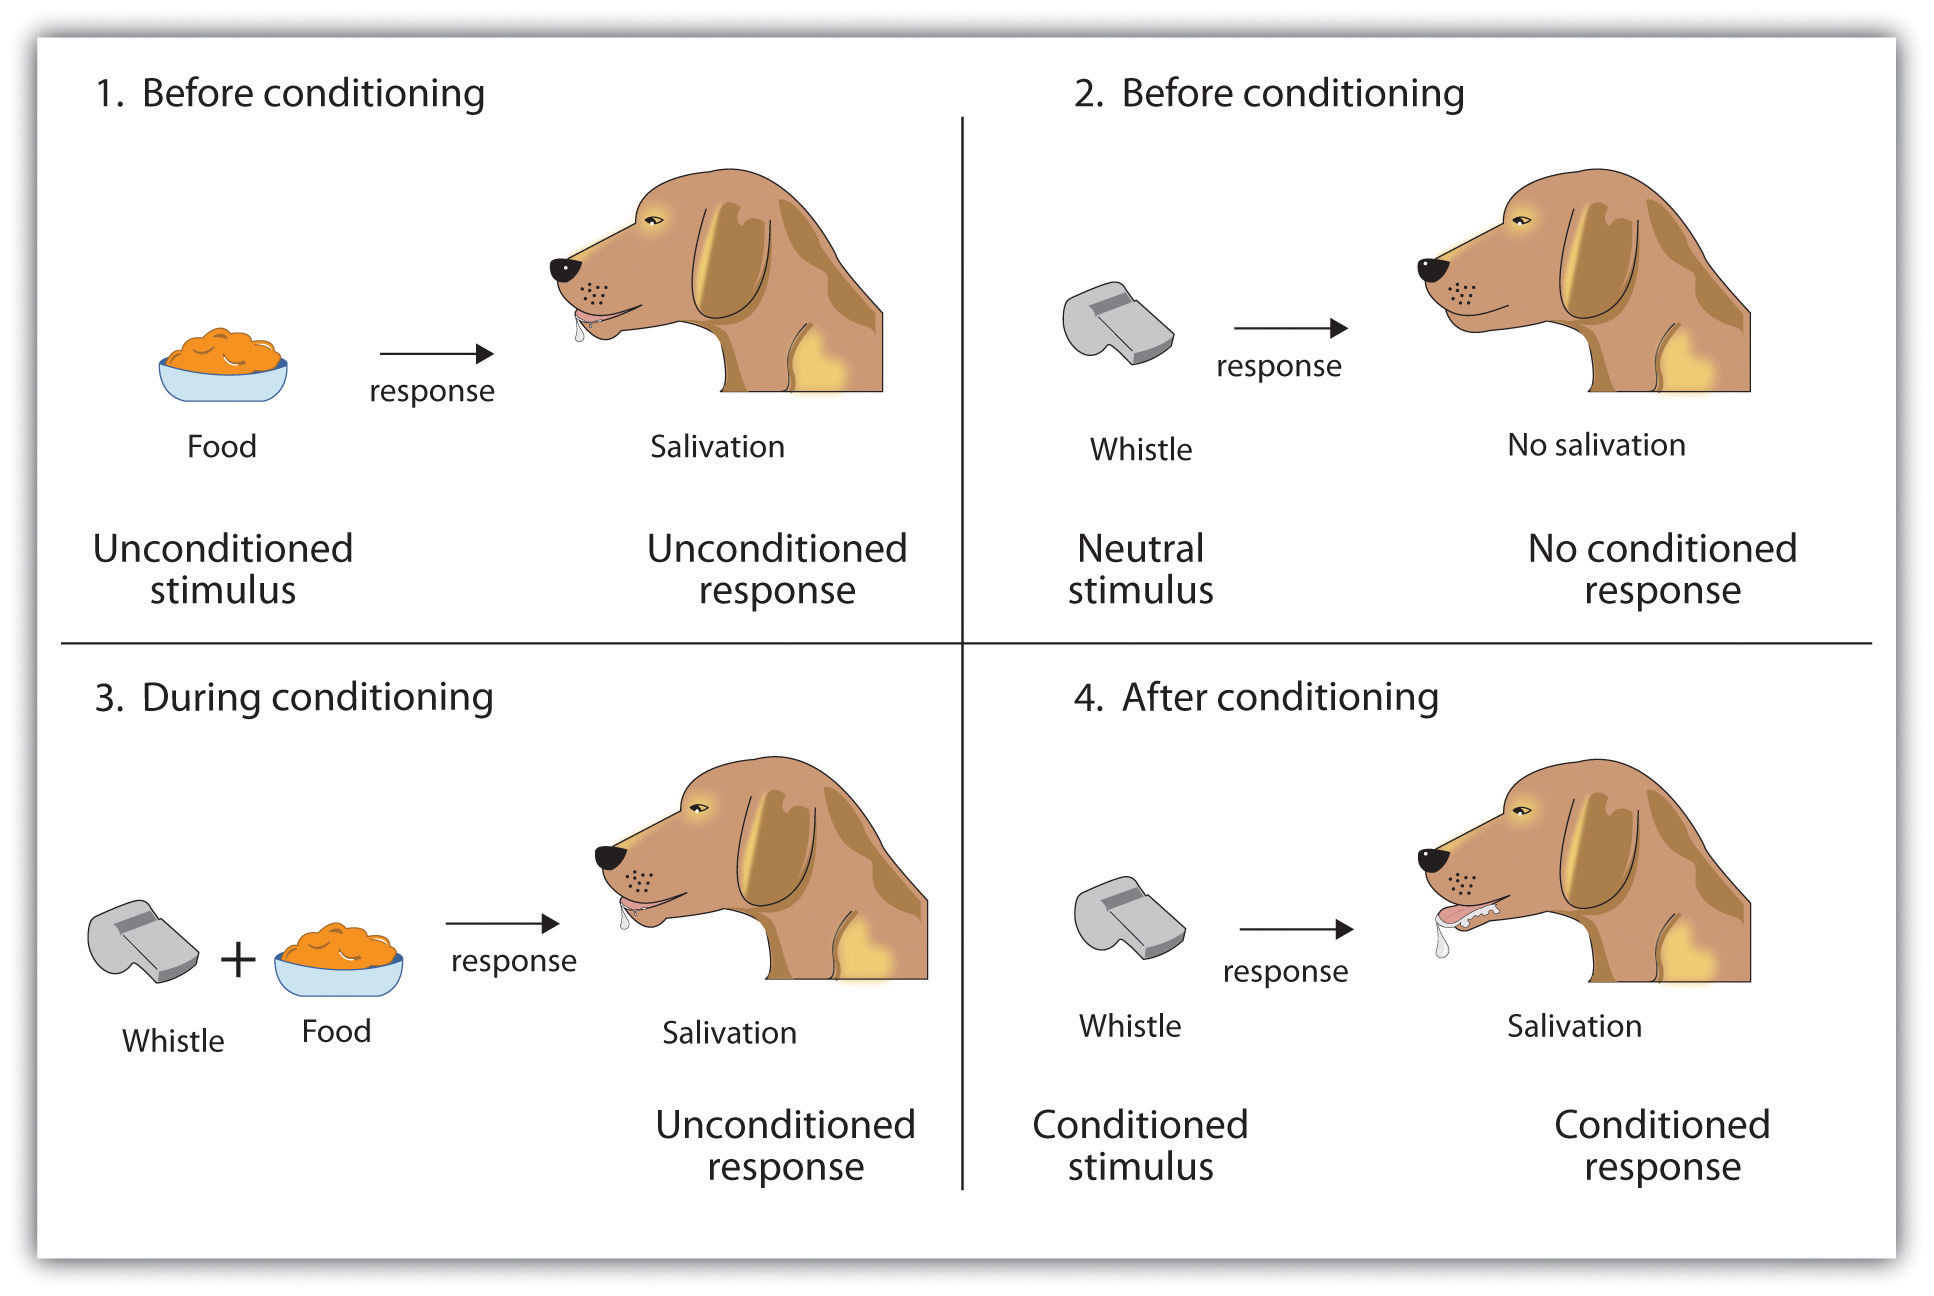
\includegraphics[scale=0.226]{WhistleAndDog.jpg}
\caption{Klasično pogojevanje piščalke namesto hrane za slinjenje pri psu~\cite{IntroductionToPsychology}.}
\label{figure:WhistleAndDog}
\end{center}
\end{figure}

Pogojevanje je evolucijsko koristno, ker omogoča organizmom razviti pričakovanja, ki jim pomagajo v dobrih in slabih okoliščinah. Razvidno je na primeru živali, ki zavoha novo hrano, jo poje in posledično zboli. Če se žival zna naučiti povezave vonja (CS) s hrano (US), se bo znala izogibati določeni hrani že po vonju.

% After he had demonstrated that learning could occur through association, Pavlov moved on to study the variables that influenced the strength and the persistence of conditioning. In some studies, after the conditioning had taken place, Pavlov presented the sound repeatedly but without presenting the food afterward. Figure 7.4, “Acquisition, Extinction, and Spontaneous Recovery” shows what happened. As you can see, after the intial acquisition (learning) phase in which the conditioning occurred, when the CS was then presented alone, the behavior rapidly decreased—the dogs salivated less and less to the sound, and eventually the sound did not elicit salivation at all. Extinction refers to the reduction in responding that occurs when the conditioned stimulus is presented repeatedly without the unconditioned stimulus.

% Although at the end of the first extinction period the CS was no longer producing salivation, the effects of conditioning had not entirely disappeared. Pavlov found that, after a pause, sounding the tone again elicited salivation, although to a lesser extent than before extinction took place. The increase in responding to the CS following a pause after extinction is known as spontaneous recovery. When Pavlov again presented the CS alone, the behavior again showed extinction until it disappeared again.

% Although the behavior has disappeared, extinction is never complete. If conditioning is again attempted, the animal will learn the new associations much faster than it did the first time.

% Pavlov also experimented with presenting new stimuli that were similar, but not identical to, the original conditioned stimulus. For instance, if the dog had been conditioned to being scratched before the food arrived, the stimulus would be changed to being rubbed rather than scratched. He found that the dogs also salivated upon experiencing the similar stimulus, a process known as generalization. Generalization refers to the tendency to respond to stimuli that resemble the original conditioned stimulus. The ability to generalize has important evolutionary significance. If we eat some red berries and they make us sick, it would be a good idea to think twice before we eat some purple berries. Although the berries are not exactly the same, they nevertheless are similar and may have the same negative properties.

% The flip side of generalization is discrimination—the tendency to respond differently to stimuli that are similar but not identical. Pavlov’s dogs quickly learned, for example, to salivate when they heard the specific tone that had preceded food, but not upon hearing similar tones that had never been associated with food. Discrimination is also useful—if we do try the purple berries, and if they do not make us sick, we will be able to make the distinction in the future. And we can learn that although the two people in our class, Courtney and Sarah, may look a lot alike, they are nevertheless different people with different personalities.

% In some cases, an existing conditioned stimulus can serve as an unconditioned stimulus for a pairing with a new conditioned stimulus—a process known as second-order conditioning. In one of Pavlov’s studies, for instance, he first conditioned the dogs to salivate to a sound, and then repeatedly paired a new CS, a black square, with the sound. Eventually he found that the dogs would salivate at the sight of the black square alone, even though it had never been directly associated with the food. Secondary conditioners in everyday life include our attractions to things that stand for or remind us of something else, such as when we feel good on a Friday because it has become associated with the paycheck that we receive on that day, which itself is a conditioned stimulus for the pleasures that the paycheck buys us.

Klasično pogojevanje obravnava samo problem napovedovanja, ker odziv živali ne vpliva na eksperiment, oziroma na splošno ne vpliva na okolje. Učenje na podlagi časovne razlike (angl. temporal difference learning), ki je opisano pozneje v razdelku~\ref{section:TD0}, je bilo prvotno povezano predvsem s klasičnim pogojevanjem in problemom napovedovanja, kjer pogojena spodbuda (CS), ki je vezana na poznejšo nepogojeno spodbudo (US), povzroči potrebo po ovrednotenju časovne razlike vrednostne funkcije. Cilj izračuna je zagotoviti, da postane pogojena spodbuda (CS) po učenju napovednik nepogojene spodbude (US). Osnutek na temo algoritmičnih pristopov do eksperimentov klasičnega pogojevanja sta sestavila Belkenius in Morén~\cite{ComputationalModelsOfClassicalConditioningAComparativeStudy}.

Čeprav je bilo učenje na podlagi časovne razlike sprva namenjeno reševanju problema napovedovanja, se uporablja tudi za reševanje problema optimalnega krmiljenja (glej razdelek~\ref{section:TD0})~\cite{ReinforcementLearningAnIntroduction}. %Zlasti omembe vredno je delo Watkinsa na Q-učenju (angl. Q-learning)~\cite{}, algoritem za krmiljenje na podlagi časovne razlike.

\subsection{Operantno pogojevanje}
V klasičnem pogojevanju se organizem nauči povezati nove spodbude z naravnim biološkim odzivom, kot je slinjenje ali strah. Organizem sam se ne nauči ničesar novega, ampak se v prisotnosti novega signala začne vesti na že obstoječi način. Po drugi strani pa gre pri operantnem pogojevanju za učenje, ki se zgodi glede na posledice vedenja in lahko vsebuje nova dejanja. Med operantno pogojevanje sodi primer, ko se pes na ukaz vsede, ker je v preteklosti za to dejanje dobil pohvalo. Za operantno pogojevanje gre tudi, ko nasilnež v šoli grozi sošolcem, ker lahko tako doseže svoje cilje, ali ko otrok domov prinese dobre ocene, ker so mu starši v nasprotnem primeru zagrozili s kaznijo. Pri operantnem pogojevanju se organizem uči iz posledic svojih dejanj.

Psiholog Edward L. Thorndike (1874-1949) je bil prvi, ki je sistematično preučil operantno pogojevanje. Izdelal je škatlo, katero je bilo mogoče odpreti samo po rešitvi preproste uganke. Vanjo je spustil mačko in opazoval njeno vedenje. Sprva so mačke praskale in grizle naključno, sčasoma pa so slučajno potisnile na ročico in odprle vrata, za katerimi je stala nagrada -- ostanki ribe. Ko je bila mačka naslednjič zaprta v škatlo, je poizkusila manjše število neučinkovitih dejanj, preden se je uspešno osvobodila. Po več poizkusih se je mačka naučila skoraj takoj pravilno odzvati.~\cite{AnimalIntelligence1}

% Thorndike puzzle box drawing.

Opazovanje tovrstnih sprememb v mačjem vedenju je Thorndikeju pomagalo razviti njegov zakon o učinku, pri katerem gre za princip, da se odzivi, ki v določeni situaciji navadno pripeljejo do prijetnega izida, bolj verjetno pojavijo ponovno v podobni situaciji, medtem ko je za odzive, ki tipično pripeljejo do neprijetnega izida, manj verjetno, da se ponovno pojavijo v tej situaciji.~\cite{AnimalIntelligence2}

Vedenjski psiholog B. F. Skinner (1904-1990) je omenjene ideje razširil in jih povezal v bolj dovršen sistem, ki opredeljuje operantno pogojevanje. Zasnoval je operantne komore (tako imenovane Skinner škatle) za sistemično preučevanje učenja, pri katerih gre za zaprto strukturoz dovolj prostora za manjšo žival, v kateri je slednja s pritiskom na palico ali gumb prišla do nagrade v obliki vode ali hrane. Struktura je poleg tega vsebovala tudi napravo za grafični zapis odzivov živali.~\cite{IntroductionToPsychology}

% Skinner box drawing.

Najosnovnejši eksperiment je Skinner izvedel na način, ki je zelo podoben Thorndikejevem poizkusu z mačkami. V škatlo je spustil podgano, katera se je sprva odzvala po pričakovanjih - hitela je naokrog, vohljala in praskala po tleh ter stenah. Čez čas je slučajno naletela na gumb in ga pritisnila ter s tem prišla do koščka hrane. Naslednjič je že potrebovala manj časa in z vsakim novim poizkusom je hitreje pritisnila na gumb. Kmalu je pritiskala na gumb, čim je lahko jedla hrano. Kot pravi zakon o učinku, se je podgana naučila ponavljati dejanje, ki ji je pomagalo priti do hrane, in prenehala z dejanjem, ki so se bila izkazala za neuspešna.~\cite{IntroductionToPsychology}

Skinner je preučeval, kako živali spreminjajo svoje vedenje v odvisnosti od okrepitve (angl. reinforcement) in kaznovanja (angl. punishment). Določil je izraze, ki razlagajo proces operantnega učenja (glej tabelo~\ref{table:OperantConditioningTerms}). Okrepitev je opredelil kot dogodek, ki utrdi ali zviša verjetnost nekega vedenja, kaznovanje pa je označil za dogodek, ki oslabi ali zniža verjetnost nekega vedenja. Uporabil je še izraza pozitivno in negativno za opredeliti, če je spodbuda predstavljena ali odvzeta. Pozitivna okrepitev torej utrdi odziv s predstavitvijo nečesa prijetnega in negativna okrepitev utrdi odziv z znižanjem ali odvzemom nečesa neprijetnega. Pohvala otroka za opravljeno domačo nalogo tako na primer sodi v pozitivno okrepitev, medtem ko predstavlja jemanje aspirina za zniževanje glavobola negativno okrepitev. V obeh primerih okrepitev zviša verjetnost, da se vedenje v prihodnosti ponovi.~\cite{IntroductionToPsychology}

% positive reinforcement, negative reinforcement
% positive punishment, negative punishment
% reinforcement = increase behavior
% punishment = decrease behavior
% positive = event response produces stimulus
% negative = event response removes stimulus
% Simply put, reinforcers serve to increase behaviors whereas punishers serve to decrease behaviors; thus, positive reinforcers are stimuli that the subject will work to attain, and negative reinforcers are stimuli that the subject will work to be rid of or to end.[9] The table below illustrates the adding and subtracting of stimuli (pleasant or aversive) in relation to reinforcement vs. punishment.
\begin{table}[htbp]
\begin{tabulary}{\textwidth}{| L | L | L | L |}
\hline
\textbf{Izraz} & \textbf{Opis} & \textbf{Izid} & \textbf{Primer} \\ \hline
Pozitivna okrepitev & Predstavljena ali povečana prijetna spodbuda & Vedenje je utrjeno & Otrok dobi slaščico, potem ko pospravi sobo \\ \hline
Negativna okrepitev & Zmanjšana ali odvzeta neprijetna spodbuda & Vedenje je utrjeno & Starši se prenehajo pritoževati, potem ko ko otrok pospravi sobo \\ \hline
Pozitivno kaznovanje & Predstavljena ali povečana neprijetna spodbuda & Vedenje je oslabljeno & Učenec dobi dodatno domačo nalogo, potem ko nagaja v razredu \\ \hline
Negativno kaznovanje & Zmanjšana ali odvzeta prijetna spodbuda & Vedenje je oslabljeno & Otrok izgubi privilegij računalnika, potem ko pride pozno domov \\ \hline
\end{tabulary}
\caption{Vpliv pozitivne in negativne okrepitve in kaznovanja na vedenje.}
\label{table:OperantConditioningTerms}
\end{table}

Čeprav je razlika med okrepitvijo (povišanje verjetnosti vedenja) in kaznovanjem (znižanje verjetnosti vedenja) navadno jasna, je v nekaterih primerih težko določiti, ali gre za pozitivno ali negativno. V vročem poletnem dnevu je lahko svež veter zaznan kot pozitivna okrepitev (ker prinese hladnejši zrak) ali pa negativna okrepitev (ker odvzame vroč zrak). V nekaterih primerih je lahko okrepitev hkrati pozitivna in negativna. Za odvisnika, jemanje drog hkrati prinese užitek (pozitivna okrepitev) in odstrani neprijetne simptome umika (negativna okrepitev).

Pomembno se je tudi zavedati, da okrepitev in kaznovanje nista zgolj nasprotna pojma. Spreminjanje vedenja s pomočjo pozitivne okrepitve je skoraj vedno učinkovitejše od kaznovanja, ker pozitivna okrepitev pri osebi ali živali izboljša razpoloženje in pripomore k vzpostavitvi pozitivnega razmerja z osebo, ki predstavlja okrepitev. Med vrste pozitivne okrepitve, ki so učinkovite v vsakdanjem življenju, sodijo izrečene pohvale in odobritve, podelitev statusa in prestiža ter neposredno denarno izplačilo. Pri kaznovanju pa je po drugi strani bolj verjetno, da bodo spremembe vedenja samo začasne, ker temelji na prisili in vzpostavi negativno ter nasprotujoče razmerje z osebo, ki predstavlja kazen. Ko se oseba, ki kazen predstavi, iz okolja umakne, se neželeno vedenje najverjetneje vrne.~\cite{IntroductionToPsychology}

Operantno pogojevanje je metoda učenja, ki se uporablja pri treniranju živali za izvajanje različnih trikov. V filmih in na predstavah so živali, od psov do konjev in delfinov, naučene dejanj z uporabo pozitivnih okrepitev -- skačejo čez ovire, se vrtijo, pomagajo osebi pri vsakdanjih opravilih in izvajajo podobna zanje neobičajna dejanja.~\cite{IntroductionToPsychology}

Velikokrat se pri učenju hkrati izvajata klasično in operantno pogojevanje. Učitelji imajo s seboj napravo, ki proizvede določen zvok. Učenje se začne z nagrajevanjem želenega enostavnega dejanja s hrano (operantno pogojevanje) in hkrati z vzpostavljanjem povezave med hrano in zvokom (klasično pogojevanje). Hrana se tako lahko po intervalih izpusti in pred dejanjem se doda še zvočni ukaz, na katerega želimo vezati učeno dejanje (klasično pogojevanje). Tako z nagrado hrane povežemo samo zvočni ukaz, ki je predstavljen pred dejanjem. Kompleksnejša dejanja se naučijo postopoma iz enostavnejših z nadaljno povezavo spodbud, kar se imenovuje proces oblikovanja.~\cite{IntroductionToPsychology}

%Spodbude, ki so organizmu naravno zadovoljive, kot na primer hrana, voda in preprečevanje bolečine, se imenujejo primarne spodbude, medtem ko gre pri sekundarni spodbudi za nevtralni dogodek, ki je s primarno spodbudo povezan s pomočjo klasičnega pogojevanja. Primer sekundarne spodbude je povezava zvoka s primarno spodbudo, kakršna je hrana. Dodaten primer vsakdanje sekundarne spodbude je denar. Denar ni zaželen sam po sebi, temveč zaradi primarnih spodbud oziroma stvari, katere se z njim lahko kupijo.~\cite{IntroductionToPsychology}

Tudi domači ljubljenčki se obnašanja naučijo na podlagi teh konceptov; ne samo na ukaz, ampak tudi samega vedenja na povodcu, do tujcev itd. S to metodo se živali lahko nauči celo razlikovati med podobnimi vzorci, s čimer lahko znanstveniki na živalih preverjajo sposobnost učenja. Porter in Neuringer~\cite{MusicDiscriminationByPigeons} sta golobe na primer naučila, da so razlikovali med različnimi vrstami glasbe, Watanabe, Sakamoto in Wakita~\cite{PigeonsDiscriminationOfPaintings} pa so jih naučili razlikovati med različnimi stili umetnosti.

Operantno pogojevanje se od klasičnega razlikuje v tem, da spremeni vedenje do okolja. Ne obravnava več samo problema napovedovanja, ampak širši problem krmiljenja.

\chapter{Problem okrepitvenega učenja} \label{chapter:Problem}
\thispagestyle{fancy}
{\em Okrepitveno učenje (angl. reinforcement learning)} po~\cite{ReinforcementLearningAnIntroduction} je učenje, kaj narediti oziroma kako izbirati dejanje, da povečamo številčni nagrajevalni signal. Učencu niso nikoli predstavljena pravilna ali optimalna dejanja, kot pri večini oblik strojnega učenja. Katera dejanja prinesejo največjo nagrado mora sam odkriti s poizkušanjem. Skozi interakcijo z okoljem se uči posledic svojih dejanj. V najbolj zanimivih in težavnih primerih imajo dejanja vpliv ne le na takojšnjo nagrado ampak tudi na naslednji položaj in posledične nagrade. Te dve značilnosti, iskanje s poizkušanjem in zakasnjene nagrade, so dve najpomembnejši lastnosti okrepitvenega učenja.

%Okrepitveno učenje ni definirano s karakterističnimi metodami učenja temveč kot karakterizacija problema učenja. Katerokoli metodo primerno za rešitev problema smatramo kot metodo okrepitvenega učenja. Celoten problem okrepitvenega učenja je predstavljen na strani \pageref{chapter:Problem}. Osnovna ideja je zajeti najpomembnejše vidike realnega problema s katerim se sooča učenec (angl. learning agent) pri interakciji s svojim okoljem za dosego cilja. Takšen učenec mora imeti nekakšna čutila za pridobivanje informacij o stanju okolja in mora biti sposoben vplivati na to stanje z dejanji. Imeti mora tudi cilj ali pa cilje, ki se nanašajo na stanje okolja. Namen opisa problema je predstaviti te vidike, čutenje, dejanje in cilj, v najenostavnejši obliki brez poenostavljenja.

Okrepitveno učenje se od nadzorovanega učenja (angl. supervised learning) razlikuje v tem, da nima izobraženega zunanjega nadzornika, ki učencu predloži primere in rezultate. Nadzorovano učenje je pomemben tip učenja, vendar pa ni primerno za učenje iz interakcije. V interaktivnih problemih je velikokrat nepraktično pridobiti primere želenega vedenja, ki so pravilni in hkrati predstavljajo vsa stanja v katerih mora učenec delovati. V neznanem okolju, kjer bi si lahko predstavljali, da je učenje najbolj koristno, se mora učenec učiti iz svojih izkušenj.

%Another key feature of reinforcement learning is that it explicitly considers the whole problem of a goal-directed agent interacting with an uncertain envi- ronment. This is in contrast with many approaches that consider subproblems without addressing how they might fit into a larger picture. For example, we have mentioned that much of machine learning research is concerned with supervised learning without explicitly specifying how such an ability would finally be useful. Other researchers have developed theories of planning with general goals, but without considering planning’s role in real-time decision- making, or the question of where the predictive models necessary for planning would come from. Although these approaches have yielded many useful results, their focus on isolated subproblems is a significant limitation.

%Reinforcement learning takes the opposite tack, starting with a complete, interactive, goal-seeking agent. All reinforcement learning agents have ex- plicit goals, can sense aspects of their environments, and can choose actions to influence their environments. Moreover, it is usually assumed from the beginning that the agent has to operate despite significant uncertainty about the environment it faces. When reinforcement learning involves planning, it has to address the interplay between planning and real-time action selection, as well as the question of how environmental models are acquired and im- proved. When reinforcement learning involves supervised learning, it does so for specific reasons that determine which capabilities are critical and which are not. For learning research to make progress, important subproblems have to be isolated and studied, but they should be subproblems that play clear roles in complete, interactive, goal-seeking agents, even if all the details of the complete agent cannot yet be filled in.

% Further, there is a focus on on-line performance, which involves finding a balance between exploration (of uncharted territory) and exploitation (of current knowledge).

To poglavje formalno definira dele okrepitvenega učenja ter določi predpostavke, ki so potrebne za opis rešitev v sledečih poglavjih.

\section{Elementi okrepitvenega učenja} \label{section:ReinforcementLearningElements}
%IS THIS THE ISSUE I HAD IN THE ALG?
%We use Rt+1 instead of Rt to denote the immediate reward due to the action taken at time t because it emphasizes that the next reward and the next state, St+1, are jointly determined.

%% agent
% learner, decision maker
% interacts with the environment to solve tasks, learning algorithms optimize his behavior, he learns
Cilj algoritmov okrepitvenega učenja je optimizirati vedenje {\em učenca (angl. agent)}. Učenec je tisti, ki se skozi interakcijo odloča o {\em dejanjih (angl. action)} za rešitev zadane {\em naloge (angl. task)}.

%% environment
% signal to the agent
% anything the agent cannot change arbitrarily is considered part of the environment
% reward computation is always external and part of the environment, the agent does not have absolute control over it
% More specifically, the agent and environment interact at each of a sequence ofdiscretetimesteps,t=0,1,2,3,....2 Ateachtimestept,theagentreceives some representation of the environment’s state, St ∈ S, where S is the set of possible states, and on that basis selects an action, At ∈ A(St), where A(St) is the set of actions available in state St. One time step later, in part as a consequence of its action, the agent receives a numerical reward , Rt+1 ∈ R, and finds itself in a new state, St+1.3 Figure 3.1 diagrams the agent–environment interaction.
% this is an abstract and flexible framework and applies to many problems
% time steps don't need to be fixed interval of time, actions could be low level controls, voltages, or high-level decisions like what school to go to or who to marry
Učenec se s svojimi dejanji vede na {\em okolje (angl. environment)}. Česar učenec ni zmožen poljubno spremeniti se smatra kot izven učenca in pripada okolju. Učenec in okolje neprestano vplivata drug na drugega; učenec izbira dejanja in okolje se nanje odziva s predstavitvijo novih {\em stanj (angl. state)} učencu. Okolje ob prehodih na nova stanja oddaja tudi številčne {\em nagrade (angl. reward)}, katere učenec skuša povečati skozi čas. Natančneje, učenec in okolje sta v interakciji v vsakem koraku diskretnega zaporedja časa $t = 0, 1, 2, 3, \dots$. V vsakem koraku učenec prejme predstavitev stanja okolja, $s_t \in S$, kjer je $S$ množica vseh možnih stanj. Glede na stanje se odloči za dejanje, $a_t \in A_s$, iz množice možnih dejanj. En časovni korak pozneje prejme učenec kot posledico svojega dejanja številčno nagrado, $r_{t+1} \in R$, in se znajde v novem stanju, $s_{t+1}$. Slika \ref{figure:AgentEnvironment} prikazuje opisan potek interakcije med učencem in okoljem. Tovrstna opredelitev elementov okrepitvenega učenja ustreza številnim težavam. Ni nujno, da časovni koraki predstavljajo fiksne intervale v resničnem času, lahko se nanašajo na poljubne zaporedne faze odločanja oziroma delovanja. Dejanja so lahko na zelo nizkem nivoju, kot na primer napetosti, ki krmilijo roko robota, ali pa na visokem nivoju, ko gre na primer za izbiranje, v katero šolo se vpisati ali pa kakšno hrano pripraviti za večerjo. Stanja so lahko tudi v zelo različnih predstavitvah, od nizkonivojskih odčitkov senzorjev do abstraktnih simboličnih opisov sob. Na splošno lahko med dejanja sodijo katerekoli odločitve, o katerih se želimo učiti, med stanja pa vse, kar nam lahko pomaga pri teh odločitvah. Edini cilj učenca je, da poveča prejete nagrade čez čas.

\begin{figure}[htbp]
\begin{center}
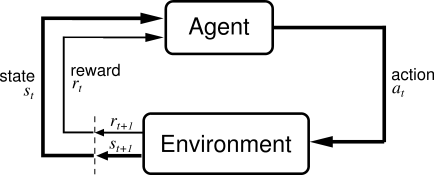
\includegraphics[scale=1.0]{AgentEnvironment.png}
\caption{Interakcija med učencem in njegovim okoljem~\cite{ReinforcementLearningAnIntroduction}.}
\label{figure:AgentEnvironment}
\end{center}
\end{figure}

%% policy
% sufficient to define behavior
% instructs the agent what to do in each state
% maps EACH state to an action
% agent uses policy to choose the next action
% This mapping is called the agent’s policy and is denoted πt, where πt(a|s) is the probability that At = a if St = s.
% correspondts to psychology's stimulus-response rules or associacions
% may be stochastic
{\em Politiko (angl. policy)} $\pi$ imenujemo pravilo po katerem se učenec odloča katero dejanje izvesti v vsakem od stanj. Z drugimi besedami: politika preslikuje stanja v dejanja. Sama po sebi zadostuje za popolno definirano vedenje. V času $t$ predstavlja $\pi_t(a_t|s_t)$ verjetnost, da učenec izvede dejanje $a_t$ v stanju $s_t$. V psihologiji koncept politike ustreza povezavam spodbud z odzivi. V splošnem so politike lahko stohastične.

%% reward function
% defines the goal, sole objective is ot maximize the reward in the long run
% maps states to rewards, scalar values, Rt element of real numbers
% indicates how well the agent is doing
% positive encourages state visits, negative discourages
% defines what is good and bad events
% in biology, it could be pleasure and pain; positive/negative simulus(?)
% may be stochastic
{\em Nagrajevalna funkcija (angl. reward function)} opredeljuje cilje v nalogi okrepitvenega učenja, saj predstavlja večanje nagrad čez čas edini učenčev cilj. V grobem, nagrajevalna funkcija stanja okolja preslikuje v realno število, $r_t$, nagrado, ki predstavlja trenutno zaželenost stanja. Pozitivne nagrade spodbujajo obiske stanj, negativne pa jih odvračajo. Oddane nagrade kažejo, kako dobro se učenec vede v okolju; nagrade opredeljujejo dobre in slabe dogodke. Uporaba nagrajevalnega signala za formalizacijo ideje cilja je ena izmed najbolj značilnih lastnosti okrepitvenega učenja. Čeprav se tovrstno oblikovanje ciljev sprva morda zdi omejujoče, se je v praksi izkazalo za zelo fleksibilno in primerno. Številne nagrade so pogosto enostavno definirane kot $+1$ ali $-1$. Bistveno je, da nagrade točno določajo zadan cilj. Nagrajevalni signal ni primerno mesto za podeljevanje učenca s predhodnim znanjem kako doseči cilj. Učenca se pri igri šaha praviloma nagradi samo v primeru zmage, ne pa za dosego podciljev, kot je zavzemanje nasprotnikovih figur. Če nagrajujemo tovrstne podcilje, se zna zgoditi, da učenec najde pot, kako doseči podcilje, ne da bi dosegel končen cilj. V primeru šaha, bi lahko našel način zavzemanja nasprotnikovih figur tudi na račun izgubljene igre. Nagrajevalna funkcija je način komuniciranja z robotom kaj naj doseže, ne pa o samem načinu, kako naj to doseže. V biološkem sistemu se nagrade lahko opredelijo kot užitek ali bolečina. V psihologiji so to okrepitve ali kaznovanje. Nagrajevalna funkcija mora obvezno biti del okolja in učenec je ne sme biti zmožen spremenjati. Na splošno so nagrajevalne funkcije lahko stohastične.

%% value function (V)
% reward function indicates what is good in an immediate sense, value function specifies what is good in the long run
% rl algorithms model this function
% maps states to values values; a state's desariability
% expresses expected reward (return?) gained from visiting the state, immediate and in the long run; the total amount an agent can expect to accumulate over the future, starting from a state
% takes into account states that are likely to follow and the rewards from those states
% make analogy to biology; long term reward
% rewards primary, values secondary, without rewards there would be no values, but we make decisions based on values
% rewards are given by the environment, values must be estimated and reestimated
% most important component of almost all rl algos is a method for efficiently estimating values
% the value function is specific to the policy
Medtem ko nagrajevalna funkcija označuje kaj je dobro v takojšnjem smislu, {\em vrednostna funkcija (angl. value function)} $V$ določa kaj je dobro na dolgi rok. Vrednostna funkcija izraža tako takojšnjo kot dolgoročno nagrado, ki se lahko pričakuje iz obiska stanja, in sicer izraža skupno količino nagrade, za katero lahko učenec predvidi, da jo bo čez čas prejel z začetkom v določenem stanju. Vrednosti upoštevajo stanja, ki si najverjetneje sledijo, in nagrade teh stanj. Vrednostna funkcija $V$ preslikuje stanja $s$ v vrednosti $v$. Najpomembnejši del skoraj vseh algoritmov okrepitvenega učenja je učinkovito ocenjevanje vrednosti. Tudi v vsakdanjem življenju velikokrat ocenjujemo in napovedujemo dolgoročno vrednost situacij, kar nam predstavlja nemajhen izziv. Stanja z visoko takojšnjo nagrado so lahko dolgoročno slaba in imajo nižjo vrednost kot alternativna. Slaščica ima na primer kratkoročen užitek, ampak pogosto ni najboljša izbira hrane kar se tiče našega telesnega zdravja. Veljati zna tudi obratno, in sicer ima stanje lahko zelo nizko takojšnjo nagrado, ampak se sčasoma izkaže za najboljšo izbiro. Naša pot do službe je lahko hitrejša, če ne izberemo najkrajše poti po dolžini, ampak upoštevamo promet do katerega nas zadana pot pripelje. Tudi živali se pri operantnem učenju učijo vrednosti in ne le takojšnjih nagrad. Hitro se naučijo, da na dolgi rok nagrade prejmejo hitreje, če se pravilno vedejo, kot pa, če se ne. Medtem ko so nagrade primarne, so vrednosti sekundarne. Brez nagrad ne bi bilo vrednosti, a vedemo se glede na ocene vrednosti. Razlika je tudi v tem, da nagrade prihajajo iz okolja, vrednosti pa moramo neprestano ocenjevati učenci sami. Vrednostna funkcija določa politiko vedenja, saj želimo s slednjim povečati nagrade, katere opisuje funkcija opisuje.

%% action value function (Q)
% same as for V, but maps states to actions
{\em Vrednostna funkcija dejanj (angl. action-value function)} $Q$ je enakovredna vrednostni funkciji z razliko, da stanja $s$ slika neposredno v dejanja $a$. Vrednostna funckija $V$ določa vrednost $v$ stanja $s$ ($V(s) = v$), medtem ko vrednostna funkcija dejanj določa vrednost $v$ dejanja $a$ ($Q(a) = v$).

%% optinal environment model
% mimics the behavior of the environment, for given state and action it predicts the next state and reward
% used for planning
% dynamic programing methods use models
% in some algorithms a model of the environment can be used, in others it's omitted
%Even if the agent has a complete and accurate environment model, the agent is typically unable to perform enough computation per time step to fully use it. The memory available is also an important constraint. Memory may be required to build up accurate approximations of value functions, policies, and models. In most cases of practical interest there are far more states than could possibly be entries in a table, and approximations must be made.
Nekateri algoritmi znajo uporabiti tudi model okolja, pri drugih je pa opuščen.

\section{Končni Markov proces odločanja}
% MARKOV REF?
V okrepitvenem učenju se učenec vede na podlagi signala iz okolja, ki ga imenujemo tudi stanje okolja. V tem razdelku je opisano kaj se zahteva od signala stanja in kakšne informacije je smiselno pričakovati od signala.

Po eni strani lahko signal stanja pove veliko več, kot samo trenutne meritve. Stanja so lahko predstavljena z močno obdelanimi originalnimi meritvami ali pa s zapletenimi strukturami, ki so zgrajene skozi čas. Ko na primer slišimo odgovor ``da'', se znajdemo v zelo različnih stanjih odvisno od predhodnega vprašanja, ki ga ne slišimo več.

Po drugi strani pa ne smemo predpostavljati, da nam signal stanja zna povedati vse o okolju, ali celo vse kar nam bi prišlo prav za odločanje. Če igramo igro s kartami ne smemo predvidevati, da bomo izvedeli kaj imajo drugi igralci v rokah ali pa katera je naslednja karta na vrhu kupa. Če učenec odgovori na telefon, ne smemo predpostavljati, da ve kdo ga kliče vnaprej. V obeh primerih obstajajo skrite informacije stanja, ki jih učenec ne more vedeti, ker jih ni nikoli prejel.

Idealno si želimo signal stanja, ki povzame vse uporabne predhodne informacije. Za to je navadno potrebna več kot samo trenutna informacija, ampak nikoli več kot celotna preteklost vseh prejetih informacij. Za signal stanja, ki zadrži vse uporabne predhodne informacije pravimo, da je {\em Markov} oziroma, da ima {\em Markovo lastnost}. Na primer, pri igri štiri v vrsto je trenutna konfiguracija vseh polj Markovo stanje, ker povzame vse pomembne informacije o poteku igre. Čeprav je veliko informacije o poteku igre izgubljene, je vse pomembno še vedno na voljo.

Pri končnem številu stanj in nagrad, je v splošnem dinamika okolja definirana samo s popolno porazdelitvijo verjetnosti
\begin{equation} \label{equation:GeneralCompleteProbabilityDistribution}
Pr\{r_{t+1} = r, s_{t+1} = s' | s_0, a_0, r_1, \dots, s_{t-1}, a_{t-1}, r_t, s_t, a_t\}
\end{equation}
na odziv okolja v času $t+1$, na dejanje v času $t$ in za vse vrednosti $r$, $s'$ in prejšnjih dogodkov $s_0, a_0, r_1, \dots, s_{t-1}, a_{t-1}, r_t, s_t, a_t$. Če ima signal stanja {\em Markovo lastnost}, pa je odziv okolja v času $t+1$ odvisen samo od stanja in dejanja v času $t$ in lahko dinamiko okolja definiramo z določitvijo le porazdelitve verjetnosti
\begin{equation} \label{equation:MarkovCompleteProbabilityDistribution}
Pr\{r_{t+1} = r, s_{t+1} = s' | s_t, a_t\},
\end{equation}
za vse $r$, $s'$, $s_t$ in $a_t$. Povedano drugače, signal stanja ima {\em Markovo lastnost} in je {\em Markovo stanje}, če in samo če je \eqref{equation:GeneralCompleteProbabilityDistribution} enako \eqref{equation:MarkovCompleteProbabilityDistribution} za vse $s'$, $r$, in preteklosti $s_0, a_0, r_1, \dots, s_{t-1}, a_{t-1}, r_t, s_t, a_t$. V tem primeru pravimo, da ima celotno okolje in naloga Markovo lastnost.

Če ima okolje Markovo lastnost, lahko iz enostavne dinamike predhodnega stanja \eqref{equation:MarkovCompleteProbabilityDistribution} napovedujemo naslednje stanje in naslednjo nagrado za trenutno stanje in dejanje. V tem okolju lahko napovedujemo vsa stanja in nagrade v prihodnosti enako dobro kot bi lahko s popolno preteklostjo do trenutnega časa. Sledi enako, da je najboljša politika izbire dejanj v Markovem stanju enako dobra kot najboljša politika izbire dejanj s trenutnim stanjem in popolno zgodovino.

Čeprav Markova lastnost velikokrat ne drži popolnoma v nalogah okrepitvenega učenja, je vseeno zelo primerno razmišljati o stanju v okrepitvenem učenju kot približnemu Markovemu stanju, saj name omogoča nam razmišljati o odločitvah in vrednostih na podlagi trenutnega stanja.

Naloga okrepitvenega učenja, ki izpolnjuje Markovo lastnost, se imenuje {\em Markov proces odločanja (angl. Markov decision process -- MDP)}. Če gre pri prostoru stanj in dejanj za končen prostor, temu pravimo {\em končen Markov proces odločanja (angl. finite MDP)}.

Končen MDP je torej popolnoma definiran s:
\begin{itemize}
\item končno množico dosegljivih stanj $S$,
\item končno množico izvedljivih dejanj $A$,
\item prehodno funkcijo, definirano na vseh stanjih iz $S$ in za vsa dejanja iz $A$, ki je za prehod v stanje $s' \in S$ odvisna samo od trenutnega stanja $s \in S$ in dejanja $a \in A$: 
\begin{equation}
P(s' | s, a) = Pr\{s_{t+1} = s' | s_t = s, a_t = a\},
\end{equation}
\item nagrajevalno funkcijo, ki je, posledično od prehodne funkcije, tudi odvisna samo od trenutnega stanja in trenutnega dejanja:
\begin{equation}
R(s, a, s') = E[r_{t+1} | s_t = s, a_t = a, s_{t+1} = s'].
\end{equation}
\end{itemize}

\section{Diskretno okrepitveno učenje}
Ta razdelek povzema okrepitveno učenje v diskretnem primeru, v katerem je prostor stanj okolja diskreten in končen, čas pa je razdeljen v diskretne korake.

Politika $\pi$ slika stanje v dejanje, kot je omenjeno v razdelku \ref{section:ReinforcementLearningElements}. Za končne MDP lahko definiramo tudi {\em optimalno politiko (angl. optimal policy)} $\pi^\star$. Naj bosta $\pi$ in $\pi^\star$ politiki in $V_\pi$ vrednostna funkcija politike $\pi$ ter $V_{\pi^\star}$ vrednostna funkcija politike $\pi^\star$. Politika $\pi^\star$ je optimalna, če ima vrednostno funkcijo  $V_{\pi^\star}$ z naslednjo lastnostjo
\begin{equation}
V_{\pi^\star}(s) >= V_\pi(s), \forall s,
\end{equation}
za vse možne politike $\pi$.

% episodic vs continuing tasks, returns, unified notation
Kar je bilo do sedaj navedeno kot pričakovana dolgoročna nagrada, se pogosto imenuje {\em pričakovan donos (angl. expected return)}. Formalna definicija donosa nekega stanja v času $t$ za poslednje nagrade $r_{t+1}, r_{t+2}, r_{t+3} \dots$ je
\begin{equation}
R_t = r_{t+1} + \gamma r_{t+2} + \gamma^2 r_{t+3} + \dots + \gamma^{T-t-1} r_T = \sum_{k=0}^{T-t-1} \gamma^k r_{t+k+1},
\end{equation}
kjer je $0 \le \gamma \le 1$. Donos je vsota vseh nadaljnjih nagrad, ki jih pričakujemo po času $t$ do končnega stanja v času $T$. V končnem stanju definiramo, da je prehod možen samo v isto stanje in nagrada ob prehodu vedno ničelna. S tem lahko poenotimo {\em epizodične} in {\em neskončne naloge} z uvedbo konstante $\gamma$, ki predstavlja {\em faktor popuščanja (angl. discount factor)}, s tem da je lahko $T = \infty$ ali $\gamma = 1$, ampak ne oboje hkrati. Pri neskončnih nalogah, ki jih ne moremo razdeliti na epizode, je $T = \infty$, saj se nikoli ne končajo, hkrati pa mora biti $\gamma < 1$, drugače lahko donos postane neskončen. Faktor popuščanja določa, koliko želimo upoštevati prihodnje nagrade. Z $\gamma = 0$ se osredotoči samo za trenutno nagrado. Pri epizodičnih nalogah, kot so igre, je navadno $\gamma = 1$.

Za končne MDP lahko {\em vrednost stanja $s$ po politiki $\pi$, t. i. vrednostno funkcijo $V_\pi(s)$}, definiramo kot pričakovan donos iz stanja $s$ z nadaljnjim upoštevanjem politike $\pi$, formalno:
\begin{equation}
V_\pi(s) = E_\pi[R_t | s_t = s] = E_\pi\left[\sum_{k=0}^\infty \gamma^k r_{t+k+1} \middle| s_t = s\right],
\end{equation}
kjer $E_\pi[.]$ predstavlja pričakovano vrednostjo, če učenec sledi politiki $\pi$.

Podobno lahko {\em vrednost dejanja $a$ v stanju $s$} po politiki $\pi$, t. i. vrednostno funkcijo dejanj $Q_\pi(s, a)$, definiramo kot pričakovan donos iz stanja $s$ ob dejanju $a$ in nadaljnjim upoštevanjem politike $\pi$, formalno:
\begin{equation}
Q_\pi(s, a) = E_\pi[R_t | s_t = s, a_t = a] = E_\pi\left[\sum_{k=0}^\infty \gamma^k r_{t+k+1} \middle| s_t = s, a_t = a\right].
\end{equation}

\section{Raziskovanje in izkoriščanje}
Eden od izzivov okrepitvenega učenja, ki jih ne najdemo v ostalih oblikah strojnega učenja, je kompromis med raziskovanjem (angl. exploration) in izkoriščanjem (angl. exploitation). Med učenjem, ko učenec uporablja približek optimalne vrednostne funkcije za svoje vedenje, mu to omogoča pridobiti največjo znano nagrado, ampak nikjer ni zagotovil, da je ta znana politika tudi v splošnem najboljša. Boljša rešitev bi mogoče lahko bila najdena, če bi učenec imel dovoljenje raziskovati dejanja, ki jih še ni poizkusil.

Spodaj opisana $\epsilon$-požrešna izbira dejanj je zelo preprosta in se v praksi pogosto uporablja. Obstaja še veliko drugih metod, nekaterih bolj kompleksnih od drugih. Več primerov je v delu Thrun~\cite{TheRoleOfExplorationInLearningControl} ter Sutton in Barto~\cite{ReinforcementLearningAnIntroduction}.

\subsection{$\epsilon$-požrešna izbira dejanj}
Eden izmed najbolj enostavnih pristopov k izbiri dejanja za ravnovesje med raziskovanjem in izkoriščanjem je uvod parametra $\epsilon$, ki določi verjetnost izbire naključnega dejanja. Po tej metodi učenec ob vsakem koraku izbere naključno dejanje z verjetnostjo $\epsilon$ in požrešno dejanje z verjetnostjo $1 - \epsilon$.

Velikokrat je koristno izbrati veliko naključnih dejanj ob začetku učenja in nato, ko učenje napreduje, znižati pogostost naključnih dejanj. S tem v fazi največjega učenja čimbolj raziščemo prostor stanj. Znižanje vrednosti $\epsilon$ logično zniža stopnjo raziskovanja in zviša stopnjo izkoriščanja. Težava pri {\em $\epsilon$-požrešni metodi izbiranja dejanj (angl. $\epsilon$-greedy action selection}) je v tem, da ne obstaja preprost način za izbiro vrednosti $\epsilon$. V veliko primerih je težko izbrati, kdaj povečati ali znižati število naključnih dejanj, ki naj jih učenec izbere.

%\section{Primeri}
%children playing with blocks
%matching shapes

% Reinforcement learning is about learning from interaction how to behave in order to achieve a goal.


%The most important feature distinguishing reinforcement learning from other types of learning is that it uses training information that evaluates the actions taken rather than instructs by giving correct actions. This is what creates the need for active exploration, for an explicit trial-and-error search for good behavior. Purely evaluative feedback indicates how good the action taken is, but not whether it is the best or the worst action possible. Evaluative feed- back is the basis of methods for function optimization, including evolutionary methods. Purely instructive feedback, on the other hand, indicates the cor- rect action to take, independently of the action actually taken. This kind of feedback is the basis of supervised learning, which includes large parts of pattern classification, artificial neural networks, and system identification. In their pure forms, these two kinds of feedback are quite distinct: evaluative feedback depends entirely on the action taken, whereas instructive feedback is independent of the action taken. There are also interesting intermediate cases in which evaluation and instruction blend together.


%1. Prediction only: RL is used to learn the value function for the policy followed. At the end of learning this value function describes for every visited state how much future reward we can expect when performing actions starting at this state.
%2. Control: By means of RL, we wish to find that particular set of policies which maximizes the reward when travelling through state space. This way we have at the end obtained an optimal policy which allows for action planning and optimal control.
%1Thus, RL also assumes that such systems “follow the Markov property”. Essentially this means that it is unimportant along which path a certain state has been reached. Once there, the state itself contains all relevant information for future calculations. Many times the Markow Property cannot be guaranteed in real world decision problem which poses practical problems when wanting to employ RL-methods. Also, we note that conventional RL needs to be augmented by additional mechanisms, if one wants to employ it to more complex, for example time and space-continuous, systems. These aspects shall not be discussed here, but see Reynolds (2002); Santos and Touzet (1999a,b).
\chapter{Tabularne rešitve} \label{chapter:TabularSolutions}
\thispagestyle{fancy}
% RL Intro has good bibliography sections for references.
V tem poglavju so opisani ključni algoritmi okrepitvenega učenja v svojih enostavnih oblikah -- ko je prostor stanj in dejanj dovolj majhen za predstavitev ocenjene vrednostne funkcije s poljem ali tabelo. V teh primerih znajo algoritmi najti optimalno vrednostno funkcijo in optimalno politiko vedenja. To je v nasprotju z aproksimacijskimi metodami opisanimi v naslednjem poglavju, katere znajo najti le približne rešitve, ampak jih lahko uporabimo učinkovito na veliko večjih problemih.

\section{Dinamično programiranje}
Richard Bellman je avtor {\em dinamičnega programiranja (angl. dynamic programming -- DP)}, izraza, ki se nanaša na zbirko algoritmov, ki jih lahko uporabimo za izračunati optimalno politiko za MDP. Algoritmi dinamičnega programiranja potrebujejo popoln in natančen model okolja za delovanje. Vsi se nanašajo na Bellmanovo enačbo \cite{OnTheTheoryOfDynamicProgramming}
\begin{align}
V_\pi(s) &= E_\pi[R_t | s_t = s] \nonumber \\
&= E_\pi\left[\sum_{k=0}^\infty \gamma^k r_{t+k+1} \middle| s_t = s\right] \nonumber \\
&= E_\pi\left[r_{t+1} + \gamma \sum_{k=0}^\infty \gamma^k r_{t+k+2} \middle| s_t = s \right] \nonumber \\
&= \sum_a \pi(a | s) \sum_{s'} P(s' | s, a) \left[R(s, a, s') + \gamma E_\pi\left[\sum_{k=0}^\infty \gamma^k r_{t+k+2} \middle| s_{t+1} = s' \right]\right] \nonumber \\
&= \sum_a \pi(a | s) \sum_{s'} P(s' | s, a) \left[R(s, a, s') + \gamma V_\pi(s')\right]. \label{equation:Bellman}
\end{align}
Bellmanova enačba pravi, da je možno izračunati vrednost vseh stanj $s$, to je, $V(s)$, z rekurzivnimi koraki čez vsa stanja ki so {\em povezana} s stanjem $s$. Izraz povezana je tukaj definiran kot: dva stanja $s$ in $s'$ sta povezana če in samo če je $P(s' | s, a) > 0$ pri vseh $a \in A$. Postopek je ponovljen za vsak $s'$ povezan s $s$ dokler ne pridemo do končnega stanja. Verjetnost $P(s' | s, a)$ določa koliko ima izraz $R(s, a, s') + \gamma V_\pi(s')$ vpliv na vrednost stanja $s$. Pomembno se je zavedati, da potrebujemo prehodno funkcijo $P$ za izračun enačbe. Če je $P$ znan se enačba razširi na sistem enačb, ki ga lahko rešimo enostaven način.

Bellman je opozoril na težavo, da se število izračunov potrebnih za rešitev sistema enačb se veča eksponentno z številom vhodnih dimenzij. Poimenoval jo je {\em prekletstvo dimenzionalnosti (angl. the curse of dimensionality)}. To je dobro znana težava v področju strojnega učenja, izvira pa iz dejstva, da se prostor stanj veča eksponentno s številom vhodnih dimenzij.

{\em Teorem izboljšanja politike (angl. policy imporvement theorem)} navaja, da ko spremenimo pot politike na pot, ki je po vrednostni funkciji boljša, dobimo izboljšano politiko. Ta lastnost je uporabljena v metodah dinamičnega programiranja tako kot tudi v veliki meri drugih algoritmov okrepitvenega učenja, vključno s algoritmi opisanimi v nadaljevanju.

\section{Monte Carlo metode}
Za razliko od DP metod, {\em Monte Carlo (MC)} metode ocenjujejo vrednostno funkcijo na podlagi interakcije z okoljem in ne potrebujejo popolnega znanja o okolju. Monte Carlo metode potrebujejo samo izkušnje -- vzorčna zaporedja stanj, dejanj in nagrad -- ki jih pridobijo med interakcijo z okoljem ali pa iz  simuliranih interakcij z okoljem. Za presenetljivo veliko aplikacij je enostavno simulirati vzorčne epizode, čeprav je težko zgraditi celoten ekspliciten model prehodnih verjetnosti, ki jih potrebujejo DP metode.

Monte Carlo metode so način rešitve problema okrepitvenega učenja z povprečenjem donosov stanj iz celotnih epizod. Ker so vrednosti stanj enostavno samo predviden donos -- predvidena nabrana zakasnjena nagrada -- z začetkom v tem stanju, lahko za oceno iz izkušenj preprosto povprečimo pridobljene donose iz tega stanja. Postopa s pridobitvijo večje količine donosov povprečje konvergira k pričakovani vrednosti. Samo po zaključku epizode so ocenjene vrednosti in politika spremenjene. Učenje je torej postopoma iz epizode do epizode in ne iz enega stanja v drugega.

Če želimo oceniti $V_\pi(s)$, vrednost nekega stanja $s$ po politiki $\pi$, imenujemo vsak pojav stanja $s$ v enem od epizod {\em obisk (angl. visit)} stanja $s$. {\em Every-visit MC metoda} oceni $V_\pi(s)$ kot povprečje donosov po vsakem obisku stanja $s$ v vsaki epizodi, {\em first-visit MC metoda} pa povpreči samo donose po prvem obisku stanja $s$ v vsaki epizodi. Oba algoritma po pravilu o velikih številih konvergirata k pričakovani vrednosti $V_\pi(s)$, ko gre število obiskov stanja $s$ v neskončnost~\cite{ReinforcementLearningWithReplacingEligibilityTraces}.

% Algoritem?

Naivna implementacija povprečenja donosov je hranitev vsakega prejetega donosa $R_t$ za vsako stanje. Nato, ko potrebujemo oceno vrednosti stanja, lahko to enostavno izračunamo z
\begin{equation}
V_t(s) = \frac{R_1 + R_2 + \dots + R_{K_s}}{K_s},
\end{equation}
kjer so $R_1, \dots, R_{K_s}$ vsi prejeti donosi v stanju $s$ pred časom $t$ in $K$ število prejetih donosov. Problem pri tej preprosti implementaciji je, da se spominske in računske zahteve večajo čez čas brez meje. Vsak nov donos po obisku stanja potrebuje več spomina za shrambo in izračun $V_t(s)$ potrebuje več časa.

% Running average.
Takšna implementacija seveda ni potrebna. Enostavno je oblikovati postopno pravilo posodobitve, ki potrebuje konstanten čas in spomin. Naj bo $V_k$ za neko stanje ocena vrednosti za $k$-ti donos, to je povprečje prvih $k - 1$ donosov. Povprečje vseh $k$ donosov lahko potem izračunamo z
\begin{align} \label{equation:RunningAverage}
V_{k+1} &= \frac{1}{k} \sum_{i=1}^k R_i \nonumber \\
&= \frac{1}{k} \left(R_k + \sum_{i=1}^{k-1} R_i\right) \nonumber \\
&= \frac{1}{k} \left(R_k + (k - 1) V_k + V_k - V_k\right) \nonumber \\
&= \frac{1}{k} \left(R_k + kV_k - V_k\right) \nonumber \\
&= V_k + \frac{1}{k} \left[R_k - V_k\right],
\end{align}
kar drži tudi za $k = 1$.

% General update rule.
To postopno pravilo posodobitve \eqref{equation:RunningAverage} je oblika, ki se pogosto uporablja v algoritmih okrepitvenega učenja, ki svoje ocene posodabljajo čez čas. Splošna oblika tega pravila je
\begin{equation}
NovaOcena \leftarrow StaraOcena + VelikostKoraka \left[Cilj - StaraOcena\right].
\end{equation}
Izraz $\left[Cilj - StaraOcena\right]$ je {\em napaka (angl. error)} v oceni vrednosti. Napako se zniža s korakom proti {\em cilju (angl. target)}. Cilj predstavlja zaželeno smer v katero bi se radi premaknili, v zgornjem primeru je to $k$-ti donos.

% Steo-size aka learning rate parameter.
Parameter {\em velikosti koraka (angl. step-size)} se v zgornji metodi spreminja v vsakem časovnem koraku ($\frac{1}{k}$). V literaturi je pogosto zaznamovan z $\alpha$ in je v intervalu ${[0, 1]}$. Imenovan je tudi {\em stopnja učenja (angl. learning rate)}, saj določa hitrost s katerim se pomaknemo proti ciljni vrednosti. V praksi je velikokrat konstanten ali pa se niža čez čas.

Enostavno pravilo posodobitve vrednosti nekega stanja $s_t$ na podlagi every-visit MC metode lahko torej opišemo z
\begin{equation}
V(s_t) \gets V(s_t) + \alpha[R_t - V(s_t)],
\end{equation}
kjer je $R_t$ dejanski donos. Monte Carlo metode počakajo dokler ni znan celoten donos stanja, preden ga uporabijo za oceno $V(s_t)$ -- počakajo do konca epizode.

Pomemben dejavnik pri MC metodah je to, da so ocene vsakega stanja neodvisne. Ocena enega stanja ne gradi na oceni kateregakoli drugega stanja, kot velja pri DP metodah. Lastnost grajenja ene ocene vrednosti na podlagi druge ocene vrednosti imenujemo {\em zagon (angl. bootstrapping)}.

%If a model is not available, then it is particularly useful to estimate action values rather than state values. With a model, state values alone are sufficient to determine a policy; one simply looks ahead one step and chooses whichever action leads to the best combination of reward and next state, as we did in the chapter on DP. Without a model, however, state values alone are not sufficient. One must explicitly estimate the value of each action in order for the values to be useful in suggesting a policy. Thus, one of our primary goals for Monte Carlo methods is to estimate q∗. To achieve this, we first consider another policy evaluation problem.

%The policy evaluation problem for action values is to estimate qπ(s,a), the expected return when starting in state s, taking action a, and thereafter following policy π. The Monte Carlo methods here are essentially the same as just presented for state values. The every-visit MC method estimates the value of a state–action pair as the average of the returns that have followed visits to the state in which the action was selected. The first-visit MC method averages the returns following the first time in each episode that the state was visited and the action was selected. These methods converge quadratically, as before, to the true expected values as the number of visits to each state–action pair approaches infinity.

Z delnim modelom okolja so vrednostne funkcije zadostne za izbiro dejanj; enostavno pogledamo naprej v katero stanje nas dejanje pelje. Brez modela pa vrednostne funkcije niso zadostne za krmiljenje. Eksplicitno moramo oceniti vrednost vsakega dejanja v vsakem stanju, da se bomo znali vesti. Ocena vrednostne funkcije dejanj, $Q(s,a)$ je v glavnem enaka, kot za $V(s)$:
\begin{equation}
Q(s_t, a_t) \gets Q(s_t, a_t) + \alpha[R_t - Q(s_t, a_t)].
\end{equation}

MacKay~\cite{IntroductionToMonteCarloMethods} povzema Monte Carlo metode v splošnem, Sutton in Barto~\cite{ReinforcementLearningAnIntroduction} pa v aplikaciji na okreptivenem učenju.

\section{Učenje na podlagi časovne razlike - TD(0)} \label{section:TD0}
{\em Učenje na podlagi časovne razlike (angl. temporal-difference -- TD)} je ena izmed osrednjih idej v okrepitvenem učenju. Medtem, ko Monte Carlo metode čakajo do konca epizode za izračun posodobitve $V(s_t)$, TD metode počakajo le en časovni korak. V času $t+1$ že tvorijo ciljno vrednosti in jo skupaj z zaznano nagrado $r_{t+1}$ in oceno $V(s_{t+1})$ uporabijo za posodobitev ocene prejšnjega stanja $V(s_t)$. Najenostavnejša TD metoda, znana kot {\em TD(0)} je
\begin{equation}
V(s_t) \gets V(s_t) + \alpha[r_{t+1} + \gamma V(s_{t+1}) - V(s_t)].
\end{equation}
Pri posodobitvi MC metode je ciljna vrednost $R_t$, pri TD pa $r_{t+1} + \gamma V_t(s_{t+1})$. Cilj posodobitvenega pravila za TD je vzet neposredno iz Bellmanove enačbe \eqref{equation:Bellman}.

Tako kot DP metoda, tudi TD uporablja zagonsko lastnost grajenja ocene vrednosti prejšnjega stanja na podlagi ocene vrednosti trenutnega stanja. Hkrati pa ima TD tudi lastnost MC metode, da ne potrebuje modela okolja. Ključna prednost TD metod je, da posodabljajo ocene iz koraka v korak napram MC metodam, ki morajo počakati na celoten donos, še posebej ko so epizode dolge.

% Algoritem TD(0).

Število 0 v TD(0) se nanaša na dejstvo, da algoritem posodobi samo vrednost enega prejšnjega stanja. Obstaja seveda tudi zelo podoben algoritem za oceno vrednosti dejanj:
\begin{equation}
Q(s_t, a_t) \gets Q(s_t, a_t) + \alpha[r_{t+1} + \gamma Q(s_{t+1}, a_{t+1}) - Q(s_t, a_t)],
\end{equation}
z imenom {\em SARSA(0) $(State_t, Action_t, Reward_{t+1}, State_{t+1}, Action_{t+1})$}.

% Zelo pomembna metoda je tudi Watkinsov {\em Q-learning} [REF], ki se direktno približuje optimalni vrednosti funkcij dejanj, neodvisno od politike vedenja:
%\begin{equation}
%Q(s_t, a_t) \gets Q(s_t, a_t) + \alpha[r_{t+1} + \gamma \max_a Q(s_{t+1}, a) - Q(s_t, a_t)].
%\end{equation}

Obe metodi konvergirata k optimalni politiki, če je $\alpha$ dovolj majhen oziroma se zmanjšuje čez čas in so vsa stanja oziroma vsi pari (stanje, dejanje) obiskani neskončno krat~\cite{LearningWithoutStateEstimationInPartiallyObservableMarkovianDecisionProcesses}.

\section{Združitev metod - TD($\lambda$)}
TD(0) glede na obiskano stanje posodobi samo vrednost prejšnjega stanja. Novost pri {\em TD($\lambda$)} algoritmu je sposobnost razširiti znanje nazaj v poljubno število vrednosti prejšnjih stanj.

Za dosego tega je uveden faktor $\lambda$ v intervalu ${[0, 1]}$, ki določa koliko daleč nazaj se znanje širi -- koliko prejšnjih stanj bomo posodabljali, oziroma s kolikšnim vplivom jih bomo posodabljali. Z $\lambda = 0$ dobimo TD(0) metodo (znanje se razširi samo na prejšnje stanje), z $\lambda = 1$ pa MC metodo (znanje se razširi na vsa prejšnja stanja). TD($\lambda$) predstavlja most med MC in TD(0) metodo. 

Splošna ciljna vrednost za TD($\lambda$) je
\begin{equation}
R_t^\lambda = (1 - \lambda) \sum_{n=1}^\infty \lambda^{n-1} R_t^{(n)},
\end{equation}
kjer je donos $R_t^{(n)}$ razširjen iz ocene vrednosti enega koraka v prihodnosti
\begin{equation}
R_t^{(1)} = r_{t+1} + \gamma V(s_{t+1})
\end{equation}
na oceno vrednosti n-tega koraka v prihodnosti
\begin{equation}
R_t^{(n)} = r_{t+1} + \gamma r_{t+2} + \gamma^2 + \dots + \gamma^{n-1} r_{t+n} + \gamma^n V(s_{t+n}).
\end{equation}
Pri MC metodi je, za primerjavo, uporabljen točen donos
\begin{equation}
R_t = r_{t+1} + \gamma r_{t+2} + \gamma^2 r_{t+3} + \dots + \gamma^{T-t-1} r_T.
\end{equation}
Ciljna vrednost predstavlja povprečje donosov za vse različne dolžine korakov, kjer je vsak donos utežen z $\lambda^{n-1}$. Normalizacijski faktor $1 - \lambda$ zagotovi, da se uteži seštejejo v vsoto~$1$. Donos enega koraka dobi največjo utež, $1 - \lambda$; donos drugega koraka dobi drugo največjo utež $(1 - \lambda)\lambda$; donos tretjega koraka dobi utež $(1 - \lambda)\lambda^2$ in tako dalje. V vsakem koraku se utež zniža za $\lambda$.

Splošno pravilo posodobitve vrednostne funkcije lahko torej podamo z
\begin{equation}
V(s_t) \gets V(s_t) + \alpha[R_t^\lambda - V(s_t)].
\end{equation}

%\begin{figure}[htbp]
%\begin{center}
%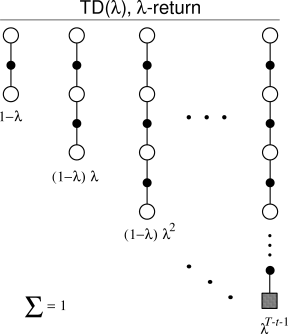
\includegraphics[scale=0.75]{LambdaReturn.png}
%\caption{Diagram uteži za TD($\lambda$)~\cite{ReinforcementLearningAnIntroduction}.}
%\label{figure:LambdaReturn}
%\end{center}
%\end{figure}

Za praktično implementacijo algoritma potrebujemo dodatno spremenljivko za vsako stanje, ki določa kolikšen vpliv bo imelo neko prihodnje dejanje na vrednost tega stanja. Te spremenljivke imenujemo {\em sledi primernosti (angl. eligibility traces)} $e$. Posodabljamo jih po pravilu {\em akumulacijskih sledi (angl. accumulating traces)}
\begin{equation}
e_t(s) = \left\{
\begin{array}{l l}
\gamma \lambda e_{t-1}(s) & \quad \textrm{če $s \ne s_t$};\\
\gamma \lambda e_{t-1}(s) + 1 & \quad \textrm{če $s = s_t$},
\end{array}
\right.
\end{equation}
ali pa {\em zamenjavnih sledi (angl. replacing traces)}
\begin{equation}
e_t(s) = \left\{
\begin{array}{l l}
\gamma \lambda e_{t-1}(s) & \quad \textrm{če $s \ne s_t$};\\
1 & \quad \textrm{če $s = s_t$},
\end{array}
\right.
\end{equation}
kjer je $\gamma$ faktor popuščanja kot je vpisano v predhodnem razdelku. Na vsakem koraku se sledi primernosti znižajo za $\gamma \lambda$, sled obiskanega stanja pa se zviša za 1 ali pa ponastavi na 1. Parameter $\lambda$ je zaradi tega imenovan tudi {\em parameter popuščanja sledi (angl. trace-decay parameter)}. Z akumulacijskimi sledmi se sled poveča za $1$ ob vsakem obisku, kar jo lahko dvigne nad vrednostjo $1$, medtem ko se pri zamenjavnih sled vedno ponastavi na 1. V poljubnem času sledi določajo katera stanja so bila nedavno obiskana. $TD(1)$ z akumulacijskimi sledmi je logično povezan z every-visit MC, $TD(1)$ z zamenjavnimi sledmi, pa z first-visit MC \cite{ReinforcementLearningWithReplacingEligibilityTraces}. Čeprav je razlika majhna, lahko zamenjavne sledi pripeljejo do znatno hitrejšega učenja~\cite{ReinforcementLearningAnIntroduction}.

Celoten algoritem $TD(\lambda)$ za napoved vrednosti z zamenjavnimi sledmi je predstavljen v tabeli \ref{table:TDLambda}. Napaka v oceni vrednosti pri TD metodah je
\begin{equation}
\delta_t = r_{t+1} + \gamma V_t(s_{t+1}) - V_t(s_t)
\end{equation}
katera se prenese na posodobitve vseh vrednosti stanj, ki imajo neničelne sledi:
\begin{equation}
\Delta V_t(s) = \alpha \delta_t e_t(s), \quad \forall s \in S.
\end{equation}

\begin{table}[htbp]
\begin{center}
\begin{tabular}{| l |}
\hline
Inicializiraj $V(s)$ poljubno \\
Za vsako epizodo: \\
\quad Inicializiraj $e(s) = 0$, $\forall s \in S$ \\
\quad Inicializiraj $s$ \\
\quad Za vsak korak: \\
\quad \quad $a \gets$ dejanje po $\pi$ za $s$ \\
\quad \quad Izvedi dejanje $a$, opazuj nagrado $r$ in naslednje stanje $s'$ \\
\quad \quad $\delta \gets r + \gamma V(s') - V(s)$ \\
\quad \quad $e(s) \gets 1$ \\
\quad \quad Za vsak $s \in S$: \\
\quad \quad \quad $V(s) \gets V(s) + \alpha \delta e(s)$ \\
\quad \quad \quad $e(s) \gets V(s) + \gamma \lambda e(s)$ \\
\quad \quad $s \gets s'$ \\
\quad dokler ni $s$ končno stanje \\
\hline
\end{tabular}
\end{center}
\caption{Algoritem TD($\lambda$) z zamenjavnimi sledmi.}
\label{table:TDLambda}
\end{table}

TD algoritem za krmiljenje {\em SARSA($\lambda$)} je iz TD($\lambda$) razvit preprosto z zamenjavo $V_t(s)$ za $Q_t(s, a)$ in $e_t(s)$ za $e_t(s,a)$, podobno kot pri SARSA(0).

% TD(λ) was proved to converge in the mean by Dayan (1992), and with probability 1 by many researchers, including Peng (1993), Dayan and Sejnowski (1994), and Tsitsiklis (1994). Jaakkola, Jordan, and Singh (1994), in addition, first proved convergence of TD(λ) under on-line updating. Gurvits, Lin, and Hanson (1994) proved convergence of a more general class of eligibility trace methods.
Singh in ostali so dokazali, da TD($\lambda$) konvergira k optimalni rešitvi~\cite{LearningWithoutStateEstimationInPartiallyObservableMarkovianDecisionProcesses}.

\chapter{Posploševanje in funkcijska aproksimacija} \label{chapter:FASolutions}
\thispagestyle{fancy}
Vsi algoritmi do sedaj so predpostavljali, da ocenjene vrednosti hranimo v tabeli, z enim vpisom za vsako vrednost. Težava je v tem, da je to mogoče le pri majhnemu številu stanj in dejanj. Ni problem samo v količini potrebnega spomina, ampak tudi v času in količini podatkov potrebnih za pravilno oceniti celotno tabelo. Potrebujemo način za posploševanje znanja iz izkušenj omejenega števila stanj.

Posploševanje je izčrpno preučeno v obliki funkcijskih aproksimacij na področju nadzorovanega učenja -- umetnih nevronskih mrežah, prepoznavi vzorcev in statističnem prilagajanju krivulj. V principu lahko uporabimo katerokoli od teh metod v okrepitvenem učenju -- posebej popularne so nevronske mreže in gradient descent metode.

\section{Nevronske mreže}
% inspired by the brain
% in comparison to other methods, they work on non-linearly separable problems
% overfitting -- early stopping and weight decay
Eden izmed najbolj zanimivih in raziskanih funkcijskih aproksimatorjev se zgleduje po najbolj spretnem posploševalcu v naravi -- možganih. {\em Umetne nevronske mreže (angl. artificial neural network)} so v splošnem predstavljene kot sistem povezanih modelov nevronov, ki znajo iz več vhodnih vrednosti izračunati eno izhodno.

{\em Nevroni} so logično povzeti kot linearna funkcija $y(\mathbf{x})$, kjer je vsaka vrednost iz vhodnega vektorja $\mathbf{x}$ utežena z vrednostjo iz {\em utežnega vektorja} $\mathbf{w}$:
\begin{equation}
y(\mathbf{x}) = \mathbf{w}^T \mathbf{x} + \omega_0.
\end{equation}
Če je vhodni vektor dvodimenzijonalen, potem utežni vektor določa orientacijo ravnine in $\omega$ {\em (angl. bias)} določa pravokotno razdaljo ravnine od središča prostora. Na funkcijo lahko gledamo tudi iz zornega kota funkcijske aproksimacije, kjer pri vhodu $\mathbf{x}$ spreminjamo $\mathbf{w}$, da dosežemo želen izhod $y(\mathbf{x})$. Pogostjo je rezultat spuščen še skozi monotonično nelinearno {\em aktivacijsko oziroma preklopno funkcijo g}:
\begin{equation}
y(\mathbf{x}) = g(\mathbf{w}^T \mathbf{x} + \omega_0).
\end{equation}
Čeprav je $g$ nelinearna funkcija, je odločitvena meja še vedno linearna, ker je $g$ monotonična.

Najpogostejši aktivacijski funkciji so sigmoidni zaradi enostavnosti izračuna njunih odvodov: logistična funkcija (zaloga vrednosti $[0, 1]$)
\begin{equation}
g(a) = \frac{1}{1 + e^{-a}}
\end{equation}
in hiperbolična tangentna funkcija (zaloga vrednosti $[-1, 1]$)
\begin{equation}
\tanh(a) = \frac{1 - e^{-2a}} {1 + e^{-2a}}.
\end{equation}
Zaradi simetrije in v splošnem boljših rezultatov pri učenju je priporočena uporaba $\tanh$~\cite{UnderstandingTheDifficultyOfTrainingDeepFeedforwardNeuralNetworks}.

%Map non-linear problem into an identical linear problem:
%\begin{equation}
%y(\mathbf{x}) = \sum_{i=1}^M w_i \phi (\mathbf{x}) + \omega_{k0}
%\end{equation}

Za učenje nevrona -- da vemo v katero smer utež spremeniti -- moramo definirati neko napako $E$ glede na izhod nevrona:
\begin{equation}
\mathbf{w_{t+1}} = \mathbf{w_t} + \alpha E \mathbf{x_t}.
\end{equation}

%This paper rigorously establishes that standard multilayer feedforward networks with as few as one hidden layer using arbitrary squashing functions are capable of approximating any Borel measurable function from one finite dimensional space to another to any desired degree of accuracy, provided sufficiently many hidden units are available. In this sense, multilayer feedforward networks are a class of universal approximators.
Posamezni nevroni se niso zmožni naučiti nelinearno ločljivih vzorcev kot je logična funkcija XOR~\cite{Perceptrons}. Če pa nevrone povežemo v {\em večnivojsko feedforward nevronsko mrežo (angl. multilayer feedforward neural network)} z vsaj tremi nivoji in dovolj velikim številom nevronov v srednjem nivoju, postane mreža univerzalni aproksimator -- poljubno natančno lahko aproksimira poljubno zvezno funkcijo, ki slika iz realnih števil v realna števila~\cite{MultilayerFeedforwardNetworksAreUniversalApproximators}. Feedforward pomeni, da mreža nima usmerjenih ciklov oziroma, da informacija iz vhodov na izhode potuje samo v eno smer.

Med probleme nevronskih mrež spadajo veliko število spremenljivk, ki jih moramo določiti empirično (število nivojev, število nevronov v vsakem nivoju, število različnih stopenj učenja), neenotna predstavitev vhodov, začetna vrednost uteži, počasna hitrost učenja, prekomerno prilagajanje (overfitting ali overtraining) in konvergiranje k lokalnem minimumu.

%\section{Metoda gradient descent}
%Gradient descent update rule:
%\begin{equation}
%\mathbf{w_{t+1}} = \mathbf{w_t} - \alpha \frac{\partial E(\mathbf{w_t})}{\partial \mathbf{w_t}}
%\end{equation}

%\begin{equation}
%\Delta \mathbf{w} = \mathbf{w_{t+1}} - \mathbf{w_t} = - \alpha \frac{\partial E(\mathbf{w_t})}{\partial \mathbf{w_t}}
%\end{equation}

%Delta rule:
%\begin{equation}
%E(\mathbf{w}) = \frac{1}{2} (v_k - y_k)^2
%\end{equation}

%\begin{equation}
%\frac{\partial E(\mathbf{w})}{\partial w_i} = -(v_k - y_k) \phi (\mathbf{x})
%\end{equation}

%\section{Multilayer neural networks}
%Backpropagation:

\section{Združitev TD($\lambda$) z nevronskimi mrežami}
Učenje na podlagi časovne razlike TD($\lambda$) lahko združimo z {\em gradient descent} metodo za izračun napake ter uporabimo {\em backpropagation} algoritem za razširitev napake po nevronski mreži~\cite{TDANNForStrategicControlProblems}.

Posodobitveno pravilo za utež nevrona v tem primeru postane
\begin{equation}
\mathbf{w_{t+1}} = \mathbf{w_t} - \alpha (R_t^\lambda - V(s_t)) \frac{\partial V(s_t)}{\partial \mathbf{w_t}}.
\end{equation}
Izraženo s sledmi primernosti:
\begin{equation}
\mathbf{w_{t+1}} = \mathbf{w_t} - \alpha \delta_t e_t,
\end{equation}
kjer je $\delta_t$ {\em TD-napaka (angl. TD-error)}
\begin{equation}
\delta_t = r_{t+1} + \gamma V(s_{t+1}) - V(s_t)
\end{equation}
in $\mathbf{e_t}$ je vektor sledi primernosti, ena sled za vsako utež v vektorju $\mathbf{w_t}$,
\begin{equation}
\mathbf{e_t} = \gamma \mathbf{\lambda e_{t-1}} + \frac{\partial V(s_t)}{\partial \mathbf{w_t}}
\end{equation}
z $\mathbf{e_0} = \mathbf{0}$.

% for linear function approximators, convergence is guaranteed if states are sampled according to the steady-state probabilities, while divergence is possible when states are sampled from distributions independent of the dynamics of the Markov chain of interest. Given that the steady-state probabilities are usually unknown, the only viable approach to generating the required samples is to perform on- line sampling. By this we mean that the samples should consist of an actual sequence of visited states obtained either through simulation of a Markov chain or observation of a physical system.
% We have run simulations in a variety of domains􏲀including a continuous gridworld􏱪 a car􏱜on􏱜the􏱜hill problem with nonlinear dynamics􏱪 and tic􏱜tac􏱜to e versus a sto chas􏱜 tic opp onent􏲀and using a variety of function approximators􏱪 including p olynomial regression􏱪 backpropagation􏱪 and lo cal weighted regression􏱝 In our exp eriments􏱪 none of these function approximators was immune from divergence􏱝
Če politika vedenja oziroma vzorčenje sledi dinamiki MDPja v interesu, potem linearni funkcijski aproksimatorji z TD($\lambda$) dokazano konvergirajo z verjetnostjo 1~\cite{AnAnalysisOfTemporalDifferenceLearningWithFunctionApproximation}. Za offline vzorčenjene in nelinearne funkcijske aproksimatorje, kot so nevronske mreže z backpropagation, pa ne obstaja zagotovil konvergence; v znatnih primerih je pokazano, da divergirajo~\cite{GeneralizationInReinforcementLearningSafelyApproximatingTheValueFunction}, čeprav obstajajo tudi empirični uspehi kot je TD-Gammon~\cite{PracticalIssuesInTemporalDifferenceLearning}.

\chapter{Učenje na namizni igri Hex} \label{chapter:Hex}
V tem poglavju so metode okrepitvenega učenja uporabljene na računalniški simulaciji namizne igre z imenom Hex. Najprej je opisana igra, njena pravila ter lastnosti, nato so predstavljene implementacije različnih metod. Na koncu poglavja so primerjani še rezultati med metodami.

\thispagestyle{fancy}
\section{Ozadje}
{\em Hex} je abstraktna potezna strategija za dva igralca, ki se igra na hexagonalni mreži, katera je navadno urejena v obliki romba. Velikost mreže je poljubna. Medtem, ko je v namizni različici pogosto v velikosti $11 \times 11$, bodo tukaj zaradi velikega števila stanj raziskane predvsem velikosti $3 \times 3$ in $4 \times 4$.

% Rules.
Vsak od igralcev ima dodeljeno eno barvo; pogoste so rdeča in modra ali pa bela in črna. Igralci izmenično zavzemajo polja eno po eno, dokler en igralec ne poveže nasprotni stranici svoje barve. Prvi igralec, ki vzpostavi povezavo med svojimi stranicami je zmagovalec.

% No draws. Favors first player.
Hex spada v kategorijo končnih (konča se v končnem številu korakov) determinističnih (brez naključnih dejavnikov) dvoigralskih iger s popolno informacijo o stanju. Igra se tudi ne more nikoli končati neodločno: edini način, da nasprotniku preprečimo povezavo stranic je s tem, da povežemo svoji stranici. Ko so stranici mreže enako dolge ima prednost prvi igralec. Ker je Hex končna igra s popolno informacijo, ki se ne more končati neodločeno, sledi da ima ali prvi ali drugi igralec zmagovalno strategijo. Če predpostavimo, da ima drugi igralec zmagovalno strategijo, jo lahko prvi igralec ``ukrade'' s tem, da naredi poljubno potezo in nato sledi zmagovalni strategiji drugega igralca. Dodatna poteza za bodisi igralca v katerem koli položaju lahko samo izboljša položaj tega igralca. Kar pomeni, da je prvi igralec v prednosti in ima on zmagovalno strategijo. Formalen dokaz je Maarup opisal v~\cite{Hex}. Ta argument samo dokazuje obstoj zmagovalne strategije brez jo opisati.

Even in Tarjan sta dokazala, da je ugotavljanje, če je določen položaj v igri Hex zmagovalen, PSPACE-polno \cite{ACombinatorialProblemWhichIsCompleteInPolynomialSpace}. Splošno je domnevano, da se PSPACE-polnih problemov ne da rešiti z učinkovitimi algoritmi (v polinomskem času).

% Number of states.


% Computational and spatial complexity.


\section{Implementacija}


\subsection{Učenec tabularne TD($\lambda)$}


\subsection{Učenec TD($\lambda$) z nevronsko mrežo}
%%%%% PONG GUY HAD MUCH BETTER SUCCESS WITH LINEAR OUPUT NEURON INSTEAD OF OTHER THINGIE.
\subsection{Naključni igralec}
% I guess I use a partial model of the environment when learning. When selecting an action I check what state that action would bring me to. I could have action-values instead, but that would be many more values and the state check is simple. Afterstates are also pretty efficient.
\section{Rezultati}
% graphs, errors; wins vs games

\chapter{Zaključek} \label{chapter:Conclusion}
\thispagestyle{fancy}
Iz okrepitvenega učenja so se razvili solidni matematični temelji in impresivne aplikacije. Računska študija okrepitvenega učenja je sedaj obsežna, z aktivnimi raziskovalci na raznolikih disciplinah kot so psihologija, teorija krmiljenja (angl. control theory), operacijske raziskave (angl. operations research), umetna inteligenca in nevroznanost. Posebej pomembne so zveze z optimalnim nadzorom in dinamičnim programiranjem. Celoten problem učenja iz interakcije za dosego ciljev ni še zdaleč rešen, vendar se je naše razumevanje na tem področju bistveno izboljšalo. Sedaj lahko postavimo sestavne ideje kot so učenje na podlagi časovne razlike, dinamično programiranje in funkcijske aproksimacije skladno s celotnim problemom.

Eden večjih trendov katerih je okrepitveno učenje deležno je večji stik med umetno inteligenco in ostalimi inženirskimi disciplinami. Nedolgo nazaj se je umetno inteligenco smatralo kot popolnoma ločeno od teorije nadzora in statistiko~\cite{ReinforcementLearningAnIntroduction}. Imelo je opravka z logiko in simboli, ne pa s števili. Umetna inteligenca so bili obširni LISP programi, ne linearna algebra, diferencialne enačbe ali statistika. V zadnjih desetletjih se je ta pogled spremenil. Moderni raziskovalci umetne inteligence sprejemajo statistične in nadzorne algoritme kot pomembne konkurenčne metode ali pa enostavno kot orodja. Prej prezrta področja med umetno inteligenco in konvencionalnega inženirstva so sedaj med najbolj aktivnimi, vključno z nevronskimi mrežami, pametnim nadzorom in okrepitvenim učenjem. V okrepitvenem učenju se ideje optimalne teorije nadora in stohastične aproksimacije razširijo za nasloviti širše in bolj ambiciozne cilje umetne inteligence.

% gpu > c > java

% while table td converges, function approximation td is tricky and not yet fully understood:
% 3.3 Scaling up in Tutorial survey and Recent Advances says something about ANN failures
% td with function approximation convergence
% td with non-linear function approximation does not converge
% some recent advances from Sutton: http://webdocs.cs.ualberta.ca/~sutton/publications.html
% Convergent Temporal-Difference Learning with Arbitrary Smooth Function Approximation

% We introduce the first temporal-difference learning algorithms that converge with smooth value function approximators, such as neural networks. Conventional temporal-difference (TD) methods, such as TD(λ), Q-learning and Sarsa have been used successfully with function approximation in many applications. How- ever, it is well known that off-policy sampling, as well as nonlinear function ap- proximation, can cause these algorithms to become unstable (i.e., the parameters of the approximator may diverge). Sutton et al. (2009a, 2009b) solved the prob- lem of off-policy learning with linear TD algorithms by introducing a new objec- tive function, related to the Bellman error, and algorithms that perform stochastic gradient-descent on this function. These methods can be viewed as natural gener- alizations to previous TD methods, as they converge to the same limit points when used with linear function approximation methods. We generalize this work to non- linear function approximation. We present a Bellman error objective function and two gradient-descent TD algorithms that optimize it. We prove the asymptotic almost-sure convergence of both algorithms, for any finite Markov decision pro- cess and any smooth value function approximator, to a locally optimal solution. The algorithms are incremental and the computational complexity per time step scales linearly with the number of parameters of the approximator. Empirical re- sults obtained in the game of Go demonstrate the algorithms’ effectiveness.
% In this paper, we solved a long-standing open problem in reinforcement learning, by establishing a family of temporal-difference learning algorithms that converge with arbitrary differentiable func- tion approximators (including neural networks). The algorithms perform gradient descent on a nat- ural objective function, the projected Bellman error. The local optima of this function coincide with solutions that could be obtained by TD(0). Of course, TD(0) need not converge with non-linear function approximation. Our algorithms are on-line, incremental and their computational cost per update is linear in the number of parameters. Our theoretical results guarantee convergence to a local optimum, under standard technical assumptions. Local optimality is the best one can hope for, since nonlinear function approximation creates non-convex optimization problems. The early empirical results obtained for computer Go are very promising. However, more practical experience with these algorithms is needed. We are currently working on extensions of these algorithms using eligibility traces, and on using them for solving control problems.

%A general gradient algorithm for temporal-difference prediction learning with eligibility traces
%ABSTRACT: A new family of gradient temporal-difference learning algorithms have recently been introduced by Sutton, Maei and others in which function approximation is much more straightforward. In this paper, we introduce the GQ(λ) algorithm which can be seen as extension of that work to a more general setting including eligibility traces and off-policy learning of temporally abstract predictions. These extensions bring us closer to the ultimate goal of this work—the development of a universal prediction learning algorithm suitable for learning experientially grounded knowledge of the world. Eligibility traces are essential to this goal because they bridge the temporal gaps in cause and effect when experience is processed at a temporally fine resolution. Temporally abstract predictions are also essential as the means for representing abstract, higher-level knowledge about courses of action, or options. GQ(λ) can be thought of as an extension of Q-learning. We extend existing convergence results for policy evaluation to this setting and carry out a forward-view/backward-view analysis to derive and prove the validity of the new algorithm.
%The GQ(λ) algorithm, which has been introduced in this paper, incorporates varying eligibility traces and option-conditional probabilities for policy evalu- ation. To derive GQ(λ), we carried out a forward- view/backward-view analysis. We extended the exist- ing convergence results to show that GQ(λ) is guaran- teed to converge to the TD(λ) fixed-point. GQ(λ) is a general gradient TD method for off-policy learning and as such can be seen as extension of Q-learning. GQ(λ) is able to learn about temporally abstract predictions, which makes it suitable to use for learning experientially grounded knowledge. In addition, GQ(λ) is online, in- cremental and its computational complexity scales only linearly with the size of features. Thus, it is suitable for large-scale applications. Our work, however, is limited to policy evaluation. Interesting future works is to ex- tend GQ(λ) for control problems and gather extensive empirical data on large-scale real-world applications.

% Interesting single layer of neurons that can learn any binary function and doesn't require much communication between neurons, continuous activation functions or calculation of derivatives
%\cite{ALearningRuleForVerySimpleUniversalApproximatorsConsistingOfASingleLayerOfPerceptrons}

Ray Kurzweil, inventor in futurist, je, v svoji nefiktivni knjigi ``The Singularity Is Near: When Humans Transcend Biology''~\cite{TheSingularityIsNear}, opisal svoj zakon o pospeševanju donosov, ki napoveduje eksponentno povečanje v tehnologijah kot so računalništvo, genetika, nanotehnologija, robotika in umetna inteligenca. Predvideva, da bo do okrog leta 2020 obstajal računalnik za tisoč ameriških dolarjev, ki bo imel računsko zmožnost posnemati človeško inteligenco. Po tem, pričakuje, da bo tehnologija optičnega zajemanja človeških možganov pripomogla k učinkovitemu modelu človeške inteligence do okrog 2025. Ta dva elementa bosta omogočala računalnikom opraviti Turingov preizkus do leta 2029. In do zgodnjih 2030 bo količina nebiološkega računanja prekoračilo zmožnost vse žive biološke inteligence človeštva. Končno eksponentno povečanje v računski zmožnosti bo privedlo do dogodka Singularnosti -- močno in moteče preoblikovanje v človeški sposobnosti -- leta 2045.

% deepmind
%\cite{PlayingAtariWithDeepReinforcementLearning}

%We present the first deep learning model to successfully learn control policies directly from high-dimensional sensory input using reinforcement learning. The model is a convolutional neural network, trained with a variant of Q-learning, whose input is raw pixels and whose output is a value function estimating future rewards. We apply our method to seven Atari 2600 games from the Arcade Learning Environment, with no adjustment of the architecture or learning algorithm. We find that it outperforms all previous approaches on six of the games and surpasses a human expert on three of them.

%http://www.theguardian.com/technology/shortcuts/2014/jan/28/demis-hassabis-15-facts-deepmind-technologies-founder-google

%http://www.technologyreview.com/news/524026/is-google-cornering-the-market-on-deep-learning/

% ANN recent advances from wiki.

\begin{thebibliography}{99}
\thispagestyle{fancy}
% Primeri:
% [1] Prvi A. Avtor, Drugi B. Avtor in Tretji C. Avtor, Naslov članka, Naslov revije 34 (2007), 24-56.
% [1] D. Marušič, R. Scapellato in B. Zgrablić, On quasiprimitive pqr-graphs, Algebra Colloq. 4 (1995), 295–314.
% [2] Prvi A. Avtor, Naslov knjige, druga izdaja. Založba, Ljubljana, 2008.
% [2] W. T. Tutte, Connnectivity in graphs, University of Toronto Press, Toronto, 1966.
% [3] Prvi A. Avtor in Drugi B. Avtor, Naslov poglavja v knjigi, v: Prvi urednik, Drugi urednik (ur.), Naslov knjige, Založba, Ljubljana, 1998, 2542–2603.
% [3] R. K. Guy, The decline and fall of Zarankiewicz's theorem, v: F. Harary (ur.), Proof Techniques in Graph Theory, Academic Press, New York, London, 1969, 63–69.

% Check capitalization of titles :\.

%\bibitem{ScienceAndHumanBehavior}
%B. F. Skinner
%\newblock{\em Science and Human Behavior},
%\newblock{Simon and Schuster, 1953}

\bibitem{SomeStudiesInMachineLearningUsingTheGameOfCheckers}
A. L. Samuel,
\newblock{\em Some Studies In Machine Learning Using the Game of Checkers},
\newblock{IBM Journal on Research and Development, 1959.}

\bibitem{TDANNForStrategicControlProblems}
A. Persson,
\newblock{\em Using Temporal Difference Methods In Combination With Artificial Neural Networks to Solve Strategic Control Problems},
\newblock{KTH Numerical Analysis and Computer Science, Royal Institute of Technology, Stockholm, Sweden, 2004.}

\bibitem{ComputationalModelsOfClassicalConditioningAComparativeStudy}
C. Balkenius, J. Morén,
\newblock{\em Computational Models of Classical Conditioning: A Comparative Study},
\newblock{From animals to animats 5: proceedings of the fifth international conference on simulation of adaptive behavior. MIT Press/Bradford Books: Cambridge, MA, 1998.}

\bibitem{AMathematicalTheoryOfCommunication}
C. E. Shannon,
\newblock{\em A Mathematical Theory of Communication},
\newblock{Bell Sys. Tech. Journal, vol. 27, 1948.}

\bibitem{IntroductionToPsychology}
C. Stangor,
\newblock{\em Introduction to Psychology},
\newblock{MIT Press, Cambridge, MA, 2011.}

\bibitem{IntroductionToMonteCarloMethods}
D. J. C. MacKay
\newblock{\em Introduction to Monte Carlo Methods},
\newblock{Learning in graphical models. Springer Netherlands, 1998.}

\bibitem{MusicDiscriminationByPigeons}
D. Porter, A. Neuringer,
\newblock{\em Music Discrimination By Pigeons},
\newblock{Journal of Experimental Psychology: Animal Behavior Processes 10.2, 1984.}

\bibitem{AnimalIntelligence1}
E. L. Thorndike,
\newblock{\em Animal Intelligence: An Experimental Study of the Associative Processes In Animals},
\newblock{Psychological Monographs: General and Applied 2.4, 1898.}

\bibitem{AnimalIntelligence2}
E. L. Thorndike,
\newblock{\em Animal Intelligence: Experimental Studies},
\newblock{The Journal of Nervous and Mental Disease 39.5, 1912.}

\bibitem{PlayingRiskAversiveGoOnALargeBoardUsingLocalNeuralNetworkPositionEvaluationFunctions}
G. Markkula,
\newblock{\em Playing risk aversive go on a large board using local neural network position evaluation functions},
\newblock{Department of physical resource theory and complex systems group, Chalmers university of technology Göteborg, 2004.}

\bibitem{PracticalIssuesInTemporalDifferenceLearning}
G. Tesauro,
\newblock{\em Practical issues in temporal difference learning},
\newblock{Machine Learning 4, 1992.}

\bibitem{ConditionedReflexes}
I. Pavlov,
\newblock{\em Conditioned Reflexes},
\newblock{Courier Dover Publications, 2003.}

\bibitem{GeneralizationInReinforcementLearningSafelyApproximatingTheValueFunction}
J. Boyan, A. W. Moore,
\newblock{\em Generalization in Reinforcement Learning: Safely Approximating the Value Function},
\newblock{Advances in neural information processing systems, 1995.}

\bibitem{AnAnalysisOfTemporalDifferenceLearningWithFunctionApproximation}
J. N. Tsitsiklis, B. Van Roy,
\newblock{\em An analysis of temporal-difference learning with function approximation},
\newblock{Automatic Control, IEEE Transactions on 42.5, 1997.}

\bibitem{MultilayerFeedforwardNetworksAreUniversalApproximators}
K. Hornik, M. Stinchcombe, H. White,
\newblock{\em Multilayer feedforward networks are universal approximators},
\newblock{Neural networks 2.5, 1989.}

\bibitem{ALearningRuleForVerySimpleUniversalApproximatorsConsistingOfASingleLayerOfPerceptrons}
P. Auer, H. Burgsteiner, W. Maass,
\newblock{\em A learning rule for very simple universal approximators consisting of a single layer of perceptrons},
\newblock{Neural Networks 21.5, 2008.}

\bibitem{PavlovianConditioningItsNotWhatYouThinkItIs}
R. A. Rescorla,
\newblock{\em Pavlovian Conditioning: It's Not What You Think It Is},
\newblock{American Psychologist, 1988.}

\bibitem{OnTheTheoryOfDynamicProgramming}
R. Bellman,
\newblock{\em On the Theory of Dynamic Programming},
\newblock{Proceedings of the National Academy of Sciences of the United States of America 38.8 1952.}

\bibitem{TheSingularityIsNear}
R. Kurzweil,
\newblock{\em The Singularity Is Near: When Humans Transcend Biology},
\newblock{Penguin, 2005.}

\bibitem{LearningToPredictByTheMethodsOfTemporalDifference}
R. S. Sutton,
\newblock{\em Learning to predict by the methods of temporal difference},
\newblock{Machine Learning 3, 1988.}

\bibitem{ReinforcementLearningAnIntroduction}
R. S. Sutton, A. G. Barto,
\newblock{\em Reinforcement Learning: An Introduction},
\newblock{MIT Press, Cambridge, MA, 1998.}

\bibitem{LearningAndBehaviorAContemporarySynthesis}
M. E. Bouton,
\newblock{\em Learning and Behavior: A Contemporary Synthesis},
\newblock{Sinauer Associates, 2007.}

\bibitem{StrategyAcquisitionForTheGameOthelloBasedOnReinforcementLearning}
M. Ito, T. Yoshioka, S. Ishii,
\newblock{\em Strategy acquisition for the game “Othello” based on reinforcement learning},
\newblock{Technical report, Nara Institute of Science and Techology, 1998.}

\bibitem{Perceptrons}
M. L. Minsky, S. A. Papert,
\newblock{\em Perceptrons - Expanded Edition: An Introduction to Computational Geometry},
\newblock{Boston, MA:: MIT press, 1987.}

\bibitem{LearningToEvaluateGoPositionsViaTemporalDifferenceMethods}
N. N. Schraudolf, P. Dayan, T. Sejnowski,
\newblock{\em Learning to evaluate go positions via temporal difference methods},
\newblock{Vol. 62 of Studies in fuzziness and soft computing, Springer Verlag, 2001.}

\bibitem{TheRoleOfExplorationInLearningControl}
S. B. Thrun,
\newblock{\em The Role of Exploration in Learning Control},
\newblock{Department of Computer Science, Carnegie-Mellon University, 1992.}

\bibitem{ACombinatorialProblemWhichIsCompleteInPolynomialSpace}
S. Even, R. E. Tarjan,
\newblock{\em A combinatorial problem which is complete in polynomial space},
\newblock{Journal of the ACM (JACM) 23.4, 1976.}

\bibitem{CognitionEvolutionAndBehavior}
S. J. Shettleworth,
\newblock{\em Cognition, Evolution and Behavior},
\newblock{Oxford University Press, 2009.}

\bibitem{ACollectionOfDefinitionsOfIntelligence}
S. Legg, M. Hutter,
\newblock{\em A Collection of Definitions of Intelligence},
\newblock{Frontiers in Aritificial Intelligence and Applications, 2007.}

\bibitem{ReinforcementLearningWithReplacingEligibilityTraces}
S. P. Singh, R. S. Sutton,
\newblock{\em Reinforcement Learning with Replacing Eligibility Traces},
\newblock{Machine learning 22.1-3, 1996.}

\bibitem{LearningWithoutStateEstimationInPartiallyObservableMarkovianDecisionProcesses}
S. P. Singh, T. Jaakkola, M. I. Jordan,
\newblock{\em Learning Without State-Estimation in Partially Observable Markovian Decision Processes},
\newblock{ICML, 1994.}

\bibitem{PigeonsDiscriminationOfPaintings}
S. Watanabe, J. Sakamoto, M. Wakita,
\newblock{\em Pigeons' Discrimination of Paintings by Monet and Picasso},
\newblock{Journal of the experimental analysis of behavior 63.2, 1995.}

\bibitem{PsychologyAStudentFriendlyApproach}
T. L. Brink,
\newblock{\em Psychology: A Student Friendly Approach},
\newblock{San Bernardino Community College, 2008.}

\bibitem{Hex}
T. Maarup,
\newblock{\em Everything you always wanted to know about Hex but were afraid to ask},
\newblock{Diss. Master’s thesis, University of Southern Denmark, 2005.}

\bibitem{PlayingAtariWithDeepReinforcementLearning}
V. Mnih, K. Kavukcuoglu, D. Silver, A. Graves, I. Antonoglou, D. Wierstra, M. Riedmiller,
\newblock{\em Playing Atari with Deep Reinforcement Learning},
\newblock{arXiv preprint arXiv:1312.5602, 2013.}

\bibitem{UnderstandingTheDifficultyOfTrainingDeepFeedforwardNeuralNetworks}
X. Glorot, Y. Bengio,
\newblock{\em Understanding the difficulty of training deep feedforward neural networks},
\newblock{International Conference on Artificial Intelligence and Statistics, 2010.}

\end{thebibliography}

%\pagestyle{fancyplain}
%\vspace*{\fill}
%     \begin{center}
%          \bf{\Huge{Priloge}}
%     \end{center}
%\vspace*{\fill}
%\thispagestyle{fancy}
%\addcontentsline{toc}{chapter}{Priloge}
%\appendix
%\appendices{A Naslov prve priloge}
%\chapter{Naslov prve priloge}
%\thispagestyle{fancy}
%Tu dodamo prvo prilogo.
%\appendices{B Naslov druge priloge}
%\chapter{Naslov druge priloge}
%\thispagestyle{fancy}
%Tu dodamo drugo prilogo.

\end{document}